\chapter{Calculus of Communicating Systems}
\label{Capitolo 4}

Fino ad ora abbiamo considerato programmi sequenziali e abbiamo studiato la loro
verifica, tramite le triple di Hoare. Si passa ora dal sequenziale al
\textbf{concorrente}. Dati due comandi $s_1$ ed $s_2$ si ha che essi sono
specificati in esecuzione concorrente con:
\[s_1|s_2\]
L'esecuzione in concorrenza può portare a diverse complicanze qualora non venga
rispettato, per esempio, un certo ordine di esecuzione. Si ha quindi il
\textbf{non determinismo}, potendo avere più risultati a seconda dell'ordine di
esecuzione. Si perde la \textbf{composizionalità}.
\begin{esempio}
  Vediamo un esempio.\\
  Siano:
  \[s_1=\{x=V\}\,\,\,x=2\,\,\,\{x=2\}\]
  \[s_2=\{x=V\}\,\,\,x=3\,\,\,\{x=3\}\]
  con $V$ indicante un valore qualunque.\\
  Posso avere:
  \[\{x=V\}\,\,\,s_1|s_2\,\,\,\{x=2\lor x=3\}\]
  avendo non determinismo.\\
  Definiamo anche:
  \[s_1'=\{x=V_0\}\,\,\,x=1;x=x+1\,\,\,\{x=2\}\]
  e vediamo, a conferma della perdita di composizionalità e determinismo che:
  \[\{x=V\}\,\,\,s_1'|s_2\,\,\,\{x=2\lor x=3\lor x=4\}\]
\end{esempio}
Si studierà quindi la \textbf{semantica della programmazione
  concorrente/parallela (o dei sistemi distribuiti)}.\\
Il problema è stato studiato da Hoare e Milner (secondo punti di vista diversi)
alla fine degli anni '70. Hoare ha introdotto un nuovo paradigma di
programmazione, il paradigma \textbf{CSP (\textit{communicating sequential
    processes})}, il linguaggio macchina dei cosiddetti \textit{transputer}. Non
si ha più una memoria condivisa ma un insieme di processi ciascuno con una sua
memoria privata. Si ha un'interazione tra processi tramite lo scambio di
messaggi del tipo \textit{hand-shacking}, avendo quindi la sincronizzazione, con
lo scambio di informazioni. Viene fatto anche un processo particolare
rappresentante la \textbf{memoria condivisa}. Avremo quindi:
\[x|s_1|s_2\]
con $x$ che rappresenta la memoria condivisa dai due processi.\\
Ad oggi diversi linguaggi di programmazione adottano una ``soluzione mista''
rispetto a questo paradigma.\\
Milner propose in modo completamente indipendente da Hoare qualcosa di molto
analogo. Milner propose infatti il \textbf{lambda calcolo
  (\textit{$\lambda$-calcolo})} per passare dal sequenziale al
concorrente. Studia in modo approfondito la composizionalità, sfruttando la
composizione tra funzioni, cercando di non perderla nel concorrente. Introduce
quindi una sorta di \textit{$\lambda$-calcolo concorrente}, introducendo il
\textbf{Calculus of Communicating Systems (\textit{CCS})}, in cui pensa ad un
calcolo algebrico per sistemi comunicanti. Adotta anche lui un paradigma che
studia un sistema (non solo dal punto di vista della programmazione) formato da
componenti, chiamati \textit{processi}. Questi processi comunicano tramite lo
scambio sincrono di messaggi, con il modello \textit{hand-shacking}. Con $a$
senza nulla indichiamo un processo generico ($a$ potrebbe essere qualsiasi cosa)
che invia e con $\overline{a}$ un processo generico che riceve.
Un sistema quindi è un insieme di processi il cui comportamento è gestito da un
calcolo algebrico, si punta alle \textbf{algebre di processi}, ovvero
linguaggi di specifica di sistemi concorrenti che si ispirano al calcolo dei
sistemi comunicanti. I messaggi di scambio corrispondono ad uno scambio di
valori di variabili e questo è rappresentabile dall'algebra. I processi possono
interagire anche con l'\textbf{ambiente esterno}. Dato un sistema $S$, si
scrive:
\[S=p_1|p_2|p_3\]
se $S$ è formato dai processi $p_1$, $p_2$ e $p_3$, processi che sono
\textit{interagenti} ``a due a due''. Ogni processo ha comunque una memoria
privata.\\ 
Grazie alla comunicazione con l'\textit{ambiente esterno} non si ha più un
\textbf{sistema chiuso}. Pnueli (che creò anche le logiche temporali) e Harvel
hanno definito questi sistemi \textbf{sistemi reattivi}, per indicare che i
sistemi reagiscono all'ambiente esterno.\\
Milner risolve il problema della \textit{composizionalità} tramite l'uso di
diverse \textit{porte} che permettono ad un processo di comunicare con altri o
con l'ambiente esterno. Quindi ogni processo può essere visto come un insieme di
sotto-processi \textit{interagenti} che però interagiscono tramite
sincronizzazione con i processi esterni tramite una porta (un sottoprocesso può
comunicare con più processi esterni tramite più porte). Bisogna comunque
mantenere il comportamento complessivo. Per il processo esterno è come se
sostituissi il processo con cui comunica con il suo sottoprocesso. Si introduce
infatti l'\textbf{equivalenza all'osservazione}, che permette di sostituire un
processo $s_i$ con $s_i'$ se sono equivalenti rispetto
all'\textit{osservazione} ovvero sse un qualsiasi osservatore esterno non è in
grado di distinguere i due processi. In questo caso \textit{osservare} significa
\textbf{interagire con il sistema} dove agisce il processo (questa è un'idea di
``osservare'' derivante dalla fisica moderna). Questo deve essere valido
\textbf{per ogni possibile osservatore}. Se questo è garantito la sostituzione
di un processo non va ad inficiare l'esecuzione complessiva, senza incorrere in
\textit{deadlock} o altre problematiche.
\begin{figure}[H]
  \centering
  % \psscalebox{1.0 1.0} % Change this value to rescale the drawing.
  % {
  %   \begin{pspicture}(0,-1.7470312)(10.48,1.7470312)
  %     \psframe[linecolor=black, linewidth=0.04, dimen=outer]
  %     (4.8,1.1378711)(0.0,-1.6621289)
  %     \psframe[linecolor=black, linewidth=0.04, dimen=outer]
  %     (4.0,0.7378711)(3.2,-0.062128905)
  %     \psframe[linecolor=black, linewidth=0.04, dimen=outer]
  %     (1.6,0.7378711)(0.8,-0.062128905)
  %     \psframe[linecolor=black, linewidth=0.04, dimen=outer]
  %     (2.8,-0.4621289)(2.0,-1.262129)
  %     \psframe[linecolor=black, linewidth=0.04, dimen=outer]
  %     (9.6,0.7378711)(7.6,-1.262129)
  %     \psline[linecolor=black, linewidth=0.04](8.4,-0.4621289)
  %     (8.4,-0.8621289)(8.8,-0.8621289)(8.8,-0.4621289)(8.4,-0.4621289)
  %     \psline[linecolor=black, linewidth=0.04](8.0,0.3378711)
  %     (8.0,-0.062128905)(8.4,-0.062128905)(8.4,0.3378711)(8.0,0.3378711)
  %     \psline[linecolor=black, linewidth=0.04](8.8,0.3378711)
  %     (8.8,-0.062128905)(9.2,-0.062128905)(9.2,0.3378711)(8.8,0.3378711)
  %     \rput[bl](0.8,1.2378711){$S$}
  %     \rput[bl](1.05,0.2478711){$p_1$}
  %     \rput[bl](3.4,0.2378711){$p_2$}
  %     \rput[bl](2.2,-0.9621289){$p_3$}
  %     \rput[bl](7.7,0.8378711){$p_2$}
  %     \psline[linecolor=black, linewidth=0.04]
  %     (1.6,0.3378711)(3.2,0.3378711)(3.2,0.3378711)
  %     \psline[linecolor=black, linewidth=0.04]
  %     (3.6,-0.062128905)(2.8,-0.8621289)
  %     \psline[linecolor=black, linewidth=0.04]
  %     (4.0,0.3378711)(5.6,0.3378711)
  %     \rput[bl](2.4,0.4378711){$x$}
  %     \rput[bl](3.2,-0.8621289){$y$}
  %     \rput[bl](5.1,0.5378711){$z$}
  %     \psline[linecolor=black, linewidth=0.04]
  %     (8.64,-0.8621289)(8.64,-1.6621289)
  %     \psline[linecolor=black, linewidth=0.04]
  %     (8.41,0.097871095)(8.8,0.097871095)
  %     \psline[linecolor=black, linewidth=0.04]
  %     (8.96,-0.062128905)(8.64,-0.3821289)
  %     \psline[linecolor=black, linewidth=0.04]
  %     (8.16,-0.062128905)(8.48,-0.3821289)
  %     \psline[linecolor=black, linewidth=0.04]
  %     (8.0,0.097871095)(7.04,0.097871095)
  %     \rput[bl](7.2,0.2578711){$x$}
  %     \rput[bl](8.8,-1.6621289){$y$}
  %     \psline[linecolor=black, linewidth=0.04]
  %     (9.18,0.097871095)(10.08,0.097871095)
  %     \rput[bl](9.72,0.2178711){$z$}
  %   \end{pspicture}
  % }
  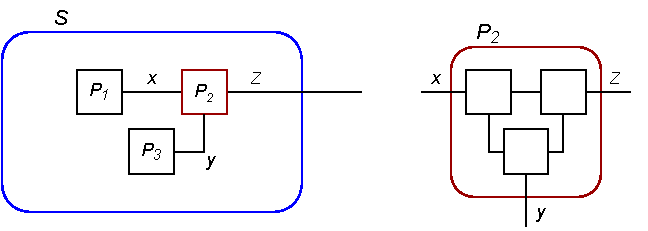
\includegraphics[scale = 0.9]{img/proc.pdf}
  \caption{Rappresentazione stilizzata di un sistema $S$ e del suo sottoprocesso
    $p_2$}
  \label{fig:proc}
\end{figure}
Vedremo quindi:
\begin{itemize}
  \item il calcolo ``puro'' di sistemi comunicanti CCS, definendone la semantica
  attraverso \textbf{Labeled Transition System, (\textit{LTS})} (\textit{sistemi
    di transizione etichettati}), (avendo come nodi i processi e archi
  etichettati dalle azioni). Useremo le operazioni ``+'', ``$\cdot$'' e la
  ricorsione, che verranno definite tramite LTS
  \item l'equivalenza all'osservazione e la \textbf{bisimulazione}. Vedremo
  anche una tecnica di verifica della \textit{bisimulazione}, tramite la
  \textbf{teoria dei giochi}
\end{itemize}
\begin{figure}
  \centering
  \begin{tikzpicture}[shorten >=1pt,node distance=2cm,on grid,auto]
    \node[state] (q_0) {$s$};
    \node[state] (q_1) [right=of q_0] {$s'$};
    \path[->]
    (q_0) edge  node {a} (q_1);
  \end{tikzpicture}
  \caption{Esempio semplice di LTS}
  \label{fig:l}
\end{figure}
\section{LTS}
\subsection{Terminologia}
\begin{shaded}
  Presa una relazione binaria $R$ su $X$, ovvero $R\subseteq X\times X$.\\
  Si ha che:
  \begin{itemize}
    \item una relazione è \textbf{riflessiva} sse $\forall x\in X$ ho che
    $(x,x)\in R$ o, scritto diversamente, $xRx$ ovvero ogni elemento è in
    relazione con se stesso 
    \item una relazione è \textbf{simmetrica} sse ho $(x,y)\in R$ allora
    $(y,x)\in R$, $\forall\,x,y\in X$
    \item una relazione è \textbf{transitiva} se ho $(x,y)\in R\land (y,z)\in R$
    allora ho $(x,z)\in R$
  \end{itemize}
  Se una relazione $R$ è simmetrica, riflessiva e transitiva allora è una
   \href{https://it.wikipedia.org/wiki/Relazione_di_equivalenza}{\textbf{relazione di equivalenza}}\footnote{Una relazione di equivalenza è un concetto matematico che esprime in termini formali quello intuitivo di "oggetti che condividono una certa proprietà".} e quindi posso ripartire $X$ in classi di
  equivalenza:
  \[[x]=\{y\in X|\,\,(x,y)\in R\}\]
  Date due classi di equivalenza $[x_1]$ e $[x_2]$ si ha che o sono uguali
  (quindi tutti gli elementi di una sono nell'altra) oppure la loro intersezione
  è vuota.\\
  Inoltre si ha che:
  \[U_{x\in X}[x]=X\]
  Si è quindi diviso $X$ in sottoinsiemi disgiunti che coprono tutto $X$.\\
  Siano $R$, $R'$ e $R''$ relazioni binarie su $X$ ($R, R',R'' \subseteq X \times X$). Si ha che:\\
  $R'$ è la \textbf{chiusura riflessiva/simmetrica/transitiva} di
  $R$ sse: 
  \begin{itemize}
    \item $R'\subseteq R$
    \item $R'$ è riflessiva/simmetrica/transitiva
    \item $R'$ è la più piccola relazione che soddisfa i primi due punti e
    quindi:
    \[\forall R''\mbox{ se }R\subseteq R''\land
      R''\mbox{riflessiva/simmetrica/transitiva}\]
    \[\mbox{allora } R'\subseteq R''\]
  \end{itemize}
\end{shaded}
\subsection{LTS come una quadrupla}
I \textbf{Labeled Transition System (\textit{LTS})} sono molto usati per
rappresentare sistemi concorrenti. Questo modello ha origine dal modello degli
automi a stati finiti, che però sono usati come riconoscitori di linguaggi.\\
Negli LTS non si ha l'obbligo di avere un insieme finito di stati.
\begin{definizione}
  Definiamo un LTS come la quadrupla:
  \[(S, Act, T, s_0)\]
  dove:
  \begin{itemize}
    \item $S$ è un insieme, anche infinito, di stati
    \item $Act$ è un insieme di nomi di \textit{azioni}
    \item $T=\{(s,a,s')\}$, con $s,s'\in S$ e $a\in Act$ oppure $T\subseteq
    S\times Act\times A$, è un insieme di triple rappresentanti le
    transizioni. Come scrittura si ha anche $(s,a,s')\in T$ oppure
    $s\stackrel{a}{\rightarrow} s'$ e quindi ho un arco etichettato con $a$ tra
    due nodi etichettati con $s$ e $s'$, come in figura \ref{fig:l}
    \item $s_0$ stato iniziale
  \end{itemize}
\end{definizione}
\begin{definizione} 
  La transizione $s\stackrel{a}{\rightarrow} s'$ può essere estesa a $w\in
  Act^*$ avendo più azioni sse:
  \begin{itemize}
    \item se $w=\varepsilon$ allora $s\equiv s'$
    \item se $w=a\cdot x,\,\,a\in Act,\,\,x\in Act^*$ sse:
    \[s\stackrel{a}{\rightarrow} s'' \mbox{ e } s''\stackrel{x}{\rightarrow}
      s'\]
  \end{itemize}
\end{definizione}
\begin{definizione}
  $s\rightarrow s'$ sse $\exists a \in Act\,\,\,\mbox{ t.c. }\,\,\,
  s\stackrel{a}{\rightarrow} s'$.\\
  Quindi:
  \[\rightarrow =\cup_{a\in Act}\stackrel{a}{\rightarrow}\]
\end{definizione}
\begin{definizione}
  $s\stackrel{*}{\rightarrow} s'$ sse $\exists w\in Act^*\mbox{ t.c. }
  s\stackrel{w}{\rightarrow} s'$. Si ha che:
  \[\stackrel{*}{\rightarrow}=\cup_{w\in Act^*}\stackrel{w}{\rightarrow}\]
  \[\stackrel{*}{\rightarrow}\subseteq S\times S\]
  La relazione $\stackrel{*}{\rightarrow}$ è la chiusura riflessiva e transitiva
  della relazione $\rightarrow$ (tale relazione non è simmetrica), avendo sempre
  $s\stackrel{*}{\rightarrow}s$ ed essendo garantita la transitività.
\end{definizione}
\section{CCS}
\begin{definizione}
  Per definire il \textbf{Calculus of Communicating Systems (\textit{CCS})}
  ``puro'' (astraendo l'aspetto delle strutture dati etc$\ldots$) dobbiamo
  definire che abbiamo: 
  \begin{itemize}
    \item $K$, ovvero un insieme di nomi di processi (\textit{buffer,
      sender,$ldots$}) che possono anche essere simboli di un alfabeto
    \item $A$, ovvero un insieme di nomi di azioni, che sono o azioni di
    sincronizzazione con l'ambiente o le componenti del sistema (anche interne
    al singolo componente)
    \item $\overline{A}$, ovvero l'insieme di nomi delle \textit{coazioni}
    contenute in $A$, $\forall\, a\in A\,\,\,\exists\,\, \overline{a}\in
    \overline{A}$, quindi:
    \[\overline{A}=\{\overline{A}|\,a\in A\}\]
    ovviamente si ha che:
    \[\overline{\overline{a}}=a\]
    \item $Act=A\cup \overline{A}\cup \{\tau\}$ dove $\tau\not\in A$ corrisponde
    all'azione di sincronizzazione tra $a$ e $\overline{a}$, ovvero la
    sincronizzazione è avvenuta. Le prime due sono \textit{azioni osservabili} e
    si indica con:
    \[\mathcal{L}=A\cup \overline{A}\]
    mentre $\tau$ non è osservabile.\\
    Ricordando che osservare un'azione significa poter interagire con essa.
  \end{itemize}
\end{definizione}
\begin{esempio}
  Vediamo un esempio.\\
  Prendiamo un sistema $S$, scuola, che eroga una lezione $\overline{lez}$ e poi
  continua ciclicamente ad erogare lezioni:
  \[S=\overline{lez}\cdot S\]
  Lo studente $ST$ segue la lezione e torna a studiare:
  \[ST=lez\cdot ST\] 
  se $S$ e $ST$ si sincronizzano ($S|ST$) lo studente osserva la lezione e il
  risultato non è più ossrvabile, essendo $\tau$.
\end{esempio}
\begin{definizione}
  I processi CCS sono di fatto operazioni CCS e un sistema CCS è definito da una
  collezione di processi $p\in K$ e si avranno:
  \[p=\mbox{espressione CCS}\]
  e si avrà solo un'equazione $\forall\,p\in K$
\end{definizione}

Definiamo meglio i processi CCS, il corrispettivo l'LTS assegnato, che sarà
del tipo:
\[(processiCCS, Act, R, p_0)\]
e, le regole d'inferenza (con premesse, eventualmente con condizioni
e con conclusioni).\\
\[CCS\to LTS\]
Dare un significato tramite LTS, regole d'inferenza e sintassi è detto
\textbf{semantica operazionale strutturale}.\\
\subsection{Regole d'inferenza per processi}
Un processo CCS può essere:
\begin{itemize}
  \item \textbf{Nil} o $0$ che ha un solo stato senza transizioni
  \begin{center}
    \begin{tikzpicture}[shorten >=1pt,node distance=2cm,on grid,auto]
      \node[state] (q_0) {$Nil$};
    \end{tikzpicture}
  \end{center}
  \item \textbf{prefisso}, in cui si ha $\alpha\cdot p,\,\alpha\in Act,\,p\in
  processi$, con la regola di inferenza:
  \[\frac{}{\alpha\cdot p\stackrel{\alpha}{\rightarrow}p}\]
  \begin{center}
    \begin{tikzpicture}[shorten >=1pt,node distance=2cm,on grid,auto]
      \node[state] (q_0) {$\alpha\cdot p$};
      \node[state] (q_1) [right=of q_0] {$p$};
      \path[->]
      (q_0) edge  node {$\alpha$} (q_1);
    \end{tikzpicture}
  \end{center}
  \item \textbf{Somma/Selezione}, $p_1+p_2,\,\,p_1,p_2\in processi$, con la regola di
  inferenza (il $+$ è la ``scelta'', come nella regex), avendo $\alpha,\beta\in
  Act$ e $p_1',p_2'\in processi$:
  \[\frac{p_1\stackrel{\alpha}{\rightarrow}p_1'}{p_1+p_2
      \stackrel{\alpha}{\rightarrow}p_1'}\] 
  \[oppure\]
   \[\frac{p_2\stackrel{\beta}{\rightarrow}p_2'}{p_1+p_2
       \stackrel{\beta}{\rightarrow}p_2'}\]
   \begin{center}
      \begin{tikzpicture}[shorten >=1pt,node distance=2cm,on grid,auto]
      \node[state] (q_0) {$p_1+p_2$};
      \node[state] (q_1) [below right=of q_0] {$p_1'$};
      \node[state] (q_2) [below left=of q_0] {$p_2'$};
      \path[->]
      (q_0) edge  node {$\alpha$} (q_1)
      (q_0) edge  node [above left] {$\beta$} (q_2);
    \end{tikzpicture}
  \end{center}
  \begin{itemize}
  \item posso avere $\sum_{i\in I}p_i$ avendo \textbf{multiple somme di
    processi}: 
  \[\frac{p_j\stackrel{\alpha}{\rightarrow}p_j'}{\sum_{i\in
        I}p_i\stackrel{\alpha}{\rightarrow}p_j'},\,j\in I\]
  e quindi se $I=\emptyset$ avrò che $\sum_{i\in I}p_i=Nil$.\\
  Posso avere non determinismo avendo $p_1=a\cdot p_1'$ e $p_2=a\cdot p_2'$,
  avendo:
   \begin{center}
      \begin{tikzpicture}[shorten >=1pt,node distance=2cm,on grid,auto]
      \node[state] (q_0) {$p_1+p_2$};
      \node[state] (q_1) [below right=of q_0] {$p_1'$};
      \node[state] (q_2) [below left=of q_0] {$p_2'$};
      \path[->]
      (q_0) edge  node {$\alpha$} (q_1)
      (q_0) edge  node[above left] {$\alpha$} (q_2);
    \end{tikzpicture}
  \end{center}
  \begin{esempio}
    Vediamo un altro esempio.
    Dati:
    \begin{itemize}
      \item $p_1=\alpha\cdot p_1'$
      \item $p_2=\beta\cdot p_2'$
      \item $p_3=\gamma\cdot p_3'$
    \end{itemize}
    \[p_1+p_2+p_3=\alpha\cdot p_1'+\beta\cdot p_2'+\gamma\cdot p_3'\]
    avendo:
    \[\frac{p_1\stackrel{\alpha}{\rightarrow}p_1'}{p_1+p_2+p_3
        \stackrel{\alpha}{\rightarrow}p_1'}\]
    \[\frac{p_2\stackrel{\alpha}{\rightarrow}p_2'}{p_1+p_2+p_3
        \stackrel{\beta}{\rightarrow}p_2'}\]
    \[\frac{p_3\stackrel{\gamma}{\rightarrow}p_3'}{p_1+p_2+p_3
        \stackrel{\gamma}{\rightarrow}p_3'}\]
    \begin{center}
      \begin{tikzpicture}[shorten >=1pt,node distance=3cm,on grid,auto]
        \node[state] (q_0) {$p_1+p_2+p_3$};
        \node[state] (q_1) [below right=of q_0] {$p_1'$};
        \node[state] (q_3) [below left=of q_0] {$p_3'$};
        \node[state] (q_2) [below =of q_0] {$p_2'$};
        \path[->]
        (q_0) edge  node {$\alpha$} (q_1)
        (q_0) edge  node[above left]{$\gamma$} (q_3)
        (q_0) edge  node[above left] {$\beta$} (q_2);
      \end{tikzpicture}
    \end{center}
  \end{esempio}
  \end{itemize}
  \item \textbf{composizione parallela}: $p_1|p_2$, avendo:
  \[\frac{p_1\stackrel{\alpha}{\rightarrow}p_1'}{p_1|p_2
      \stackrel{\alpha}{\rightarrow}p_1'|p_2}\]
  \[oppure\]
  \[\frac{p_2\stackrel{\alpha}{\rightarrow}p_2'}{p_1|p_2
      \stackrel{\alpha}{\rightarrow}p_1|p_2'}\]
  \[oppure\]
  \[\frac{p_1\stackrel{\alpha}{\rightarrow}p_1'\land p_2
      \stackrel{\overline{\alpha}}{\rightarrow}p_2'}{p_1|p_2
      \stackrel{\tau}{\rightarrow}p_1'|p_2'}\]
  e quindi, in quest'ultimo caso, non potremo più avere altre
  sincronizzazioni. \\
  Quindi avendo $p_1=a\cdot p_1'$ e $p_2=a\cdot p_2'$ ho che $p_1|p_2$
  corrisponde a $a\cdot p_1'|\overline{a}\cdot p_2'$, e, l'LTS corrisponde a:
  \begin{center}
    \begin{tikzpicture}[shorten >=1pt,node distance=3cm,on grid,auto]
      \node[state] (q_0) {\small{$a\cdot p_1'|\overline{a}\cdot p_2'$}};
      \node[state] (q_1) [below right=of q_0] {\small{$a\cdot p_1'|p_2'$}};
      \node[state] (q_3) [below left=of q_0] {\small{$p_1'|\overline{a}\cdot
          p_2'$}};
      
      \node[state] (q_2) [below right =of q_3] {\small{$p_1'|p_2'$}};
      \path[->]
      (q_0) edge  node {$\overline{a}$} (q_1)
      (q_1) edge  node {$a$} (q_2)
      (q_3) edge  node [below left]{$\overline{a}$} (q_2)
      (q_0) edge  node [above left]{$a$} (q_3)
      (q_0) edge  node [above left] {$\tau$} (q_2);
    \end{tikzpicture}
  \end{center}
  \item \textbf{restrizione}, sia $L\subseteq A$. Si ha che:
  \[P_{\backslash L}\]
  Si dice che \textit{"P è ristretto ad L"}, il ché significa che il processo $P$ non può interagire con il suo ambiente con
  azioni in $L\cup \overline{L}$ poiché le azioni in $L\cup \overline{L}$ sono
  locali a $P$. Avendo quindi:
  \[\frac{p\stackrel{\alpha}{\rightarrow}p'}{P_{\backslash L}
      \stackrel{\alpha}{\rightarrow}p'_{\backslash L}}
    ,\,\alpha,\overline{\alpha}\not\in L,\,\,L\subseteq A\]
    \textbf{NOTA:} se non si può effettuare $a$ allora non si può neanche effettuare $\overline{a}$. Posso eseguire entrambe solo durante la sincronizzazione.

  \item \textbf{rietichettatura}, ovvero il cambiamento di nome a una
  componente, a una certa azione, per poter riusare tale nome. Ho quindi una
  funzione $f$ tale che:
  \[F:Act\to Act\]
  inoltre devo avere sempre garantito che:
  \begin{itemize}
    \item $f(\tau)=\tau$, ovvero le $\tau$ non cambiano
    \item $f(\overline{a})=\overline{f(a)}$ quindi un'azione soprassegnata può
    cambiare nome solo in un'altra soprassegnata. \\ Quindi \[a\to \overline{x} \iff \overline{a}\to x\]
  \end{itemize}
  Ho quindi $p_{[f]}$ tale che:
  \[\frac{p\stackrel{\alpha}{\rightarrow}p'}{p_{[f]}
      \stackrel{f(\alpha)}{\rightarrow}p'_{[f]}}\]
  Ho quindi che:
  \[\frac{p\stackrel{\alpha}{\rightarrow}p'}{k
      \stackrel{\alpha}{\rightarrow}p'}\iff k=p\]
\end{itemize}
Quindi dato un CCS posso associare un LTS per quanto riguarda la semantica.\\
\subsection{Precedenza degli operatori}
Si ha una \textbf{precedenza degli operatori}, da quello con più precedenza a
quello con meno precedenza: 
\begin{enumerate}
  \item restrizione
  \item rietichettatura
  \item prefisso
  \item composizione parallela
  \item somma
\end{enumerate}
\begin{esempio}
  Avendo:
  \[R+a\cdot p\,\,|\,\,b\cdot Q_{\backslash L}\]
  sarebbe:
  \[R+((a\cdot p)\,\,|\,\,b\cdot(Q_{\backslash L}))\]
\end{esempio}
\begin{esempio}
\[S=(P1|B1|C1)_{\backslash \{dep,est\}}\]
\[
\begin{cases} 
    P1 = prod \cdot P2\\
    B1 = dep \cdot B2\\
    C1 = est \cdot C2\\
    P2 = \overline{dep} \cdot P1\\
    B2 = \overline{est} \cdot B1\\
    C2 = con \cdot C1\\
\end{cases} 
\]
  \begin{center}
    \begin{tikzpicture}[shorten >=1pt,node distance=5cm,on grid,auto]
     \node[state] (p1b1c1) {$(P1|B1|C1)_{\backslash \{dep,est\}}$}; 
     
      \node[state] (p1b1c2) [right=of p1b1c1] {$(P1|B1|C2)_{\backslash \{dep,est\}}$};
      
      \node[state] (p1b2c1) [above=of p1b1c1]
      {$(P1|B2|C1)_{\backslash \{dep,est\}}$};
      
      \node[state] (p2b1c1) [right=of p1b2c1] {$(P2|B1|C1)_{\backslash \{dep,est\}}$};
      
      \node[state] (p1b2c2) [above=of p1b2c1]
      {$(P1|B2|C2)_{\backslash \{dep,est\}}$};
      
        \node[state] (p2b2c1) [right=of p1b2c2] 
      {$(P2|B2|C1)_{\backslash \{dep,est\}}$};
      
        \node[state] (p2b1c2) [above=of p1b2c2] 
      {$(P2|B1|C2)_{\backslash \{dep,est\}}$};
      
            \node[state] (p2b2c2) [right=of p2b1c2] 
      {$(P2|B2|C2)_{\backslash \{dep,est\}}$};
      
      \path[->]
      (p1b1c1) edge [right] node {$prod$} (p2b1c1);
      (p2b1c1) edge [right] node {$\tau$} (p1b2c1);
      (p1b2c1) edge [right]  node {$prod$} (p2b2c1);
      (p1b2c1) edge [right]  node {$\tau$} (p1b1c2);
      (p1b1c2) edge [right]  node {$prod$} (p2b1c2);
      (p1b1c2) edge [right]  node {$con$} (p1b1c1);
      (p2b2c1) edge [right] node {$\tau$} (p1b1c2);
      (p2b1c2) edge [right] node {$con$} (p2b1c1);
    \end{tikzpicture}
  \end{center}
\end{esempio}
\begin{esempio}
  Si ha:
  \[a\cdot Nil\,\,|\,\,\overline{a}\cdot Nil\]
  ovvero:
  \begin{center}
    \begin{tikzpicture}[shorten >=1pt,node distance=4cm,on grid,auto]
      \node[state] (q_0) {\footnotesize{$a\cdot Nil\,\,|\,\,\overline{a}\cdot
          Nil$}}; 
      \node[state] (q_1) [below right=of q_0] {\footnotesize{$a\cdot
          Nil\,\,|\,\,Nil$}};  
      \node[state] (q_3) [below left=of q_0]
      {\footnotesize{$Nil\,\,\,\,|\,\,\overline{a}\cdot Nil$}}; 
      \node[state] (q_2) [below right =of q_3] {\footnotesize{$Nil|Nil$}};
      \path[->]
      (q_0) edge  node {$\overline{\alpha}$} (q_1)
      (q_1) edge  node {$\alpha$} (q_2)
      (q_3) edge  node [below left]{$\overline{\alpha}$} (q_2)
      (q_0) edge  node [above left]{$\alpha$} (q_3)
      (q_0) edge  node [above left] {$\tau$} (q_2);
    \end{tikzpicture}
  \end{center}
  Posso quindi eseguire le due operazioni o in una sequenza o nell'altra.\\
  Ho quindi una \textbf{simulazione sequenziale non deterministica} del
  comportamento del sistema dato dalla composizione parallela.
\end{esempio}
Quanto visto in questo esempio è possibile perché nell'ipotesi di Milner si ha
che $a$ e $\overline{a}$ sono \textbf{operazioni atomiche}.\\
Si hanno anche modelli di CCS modellati con:
\begin{itemize}
  \item reti di Petri
  \item strutture ad eventi
\end{itemize}
ovvero due modelli in cui si considera la semantica basata sulla \textbf{true
  concurrency}, a \textit{ordini parziali}, ovvero non si impongono sequenze
quindi due processi o si sincronizzano o vengono eseguiti in modo concorrente.
\begin{esempio}
  Costruisco il sistema di transizioni della specifica:
  \[S=\overline{lez}\cdot S\]
  \begin{center}
    \begin{tikzpicture}[shorten >=1pt,node distance=2cm,on grid,auto]
      \node[state] (q_0) {$S$};
      \path[->]
      (q_0) edge [loop right]  node {$\overline{lez}$} (q_0);
    \end{tikzpicture}
  \end{center}
  avendo:
  \[Uni=(M|LP)_{\{\backslash coin, caffe\}}\]
  Ho,seguendo nei vari step le regole di inferenza legate alla
  sincronizzazione:
  
  \[(coin\cdot \overline{caffe}\cdot
    M\,\,|\,\,\overline{lez}\cdot\overline{coin}\cdot caffe\cdot
    LP)_{\{\backslash coin, caffe\}}\]
  eseguo $\overline{lez}$ passo a:
  \[(coin\cdot \overline{caffe}\cdot
    M\,\,|\,\,\overline{coin}\cdot caffe\cdot
    LP)_{\{\backslash coin, caffe\}}\]
  sincronizzo con $coin$ e quindi passo con $\tau$:
  \[(\overline{caffe}\cdot
    M\,\,|\,\, caffe\cdot
    LP)_{\{\backslash coin, caffe\}}\]
  sincronizzo con $caffe$ e quindi passo con $\tau$:
   \[(coin\cdot \overline{caffe}\cdot
    M\,\,|\,\,\overline{lez}\cdot\overline{coin}\cdot caffe\cdot
    LP)_{\{\backslash coin, caffe\}}\]
  tornando all'inizio.\\
  (in realtà avrei i nodi per ogni formula e gli archi etichettati prima con
  $\overline{lez}$ e poi con $\tau$ per gli ultimi due)\\
  (\textbf{I due $\tau$ non possono avvenire ottemperantemente}).\\
  
\end{esempio}
\begin{esercizio}
  Costruire LTS relativo a:
  \[X=((a\cdot p_1'+\overline{b}\cdot p_1'')|(\overline{a}\cdot P_2'+b\cdot
    p_2''))_{\{a\}}\]
  (nessuno può quindi interagire con l'ambiente tramite $a$ e $\overline{a}$)
  \begin{center}
    \begin{tikzpicture}[shorten >=1pt,node distance=5cm,on grid,auto]
     \node[state] (q_0) {$X$}; 
      \node[state] (q_1) [left=of q_0] {$(p_1'|p_2')_{\{a\}}$};
      
      \node[state] (q_2) [below right=of q_0]
      {$(p_1''|(\overline{a}\cdot p_2'+b\cdot p_2''))_{\{a\}}$};
      \node[state] (q_3) [below left=of q_0]
      {$((a\cdot p_1'+\overline{b}\cdot p_1'')|p_2'')_{\{a\}}$};
      \node[state] (q_4) [below left=of q_2]
      {$(p_1''|p_2'')_{\{a\}}$};
      
      \path[->]
      (q_0) edge  node {$\overline{b}$} (q_2)
      (q_0) edge [above] node {$\tau$} (q_1)
      (q_2) edge [above left] node {$b$} (q_4)
      (q_3) edge  node {$\overline{b}$} (q_4)
      (q_0) edge  node {$\tau$} (q_4)
      (q_0) edge [above left] node {$b$} (q_3);
    \end{tikzpicture}
  \end{center}
\end{esercizio}
Posso infine chiedermi, vedendo l'esempio sopra, se $Uni$ implementa $S$, vista
come specifica. Quindi mi chiedo se posso quindi sostituire $S$ con $Uni$.\\
Innanzitutto per poter dire che una certa implementazione soddisfa (indicata con
$implementazione \vDash specifica$) una certa
specifica o se due implementazioni diverse soddisfano la stessa specifica ci
serve una \textbf{relazione di equivalenza} tra processi CCS, ovvero una $R$:
\[R\subseteq P_{CCS}\times P_{CCS}\]
che sia:
\begin{itemize}
  \item riflessiva
  \item simmetrica
  \item transitiva
\end{itemize}
Bisognerà inoltre astrarre:
\begin{itemize}
  \item gli stati e considerare le azioni $Act$
  \item dalle sincronizzazioni interne, ovvero dalle $\tau$
  \item rispetto al non determinismo
\end{itemize}
Milner poi asserisce che $R$ deve essere inoltre una \textbf{congruenza}
rispetto agli operatori del CCS.\\
\begin{definizione}
  Una relazione di equivalenza $R$ è una \textbf{congruenza} sse:
  \[\forall \,\,p,q\in Proc_{CCS} \land \forall c[\cdot] \mbox{ contesto CCS}\]
  (avendo quindi un contesto CCS sostituibile con qualcosa)\\
  allora:
  \[\mbox{se }pRq\mbox{ allora si ha }c[p]\,R\,\,c[q]\]
\end{definizione}
\begin{esempio}
  Preso $Uni=(M\,\,|\,\,LP)_{\{caffe,coin\}}$ posso dire che prendo il contesto:
  \[(\cdot\,\,|\,\,LP)_{\{caffe,coin\}}\]
  se $M_1\,R\,M_2$ allora deve succedere che:
  \[(M_1\,\,|\,\,LP)_{\{caffe,coin\}}\,R\,\,(M_2\,\,|\,\,LP)_{\{caffe,coin\}}\]
  quindi posso sostituire l'uno con l'altro senza avere conseguenze, essendo
  equivalenti.
\end{esempio}
\begin{teorema}
  Dati due processi $p_1$ e $p_2$ a cui assegniamo i due LTS $v_1$ e $v_2$. I
  due processi sono equivalenti se $v_1$ e $v_2$ sono isomorfi. Possiamo in
  realtà cercare qualcosa di ``meno forte'' rispetto all'isomorfismo ma che
  garantisca lo stesso risultato.\\
  Si va a vedere quindi se i due LTS \textbf{ammettono le stesse sequenze di
    operazioni}, prendendo l'\textbf{equivalenza forte} tra automi a stati
  finiti. Questa è detta \textbf{equivalenza rispetto alle tracce} (che vale
  anche per due programmi, che sono equivalenti se implementano la stessa
  sequenza di istruzioni, lo stesso algoritmo). \textit{È comunque più forte di
    dire che hanno la stessa pre-condizione e post-condizione.}\\
  \textbf{Bisognerà discutere la cosa rispetto alla congruenza}.\\
   Preso $p\in Proc_{CCS}$ ho l'insieme delle traccie di $p$:
  \[tracce(p)=\{w\in Act^*|\,\exists\,p'\in Proc_{CCS}
    \,\,p\stackrel{w}{\rightarrow} p'\}\]
  \textit{Suppongo, per ora, di non considerare le sincronizzazioni (quindi
    senza $\tau$).} 
\end{teorema}
\begin{teorema}
  Preso $p'\in Proc_{CCS}$ ho che è equivalente rispetto alle tracce a $p''$,
  scritto:
  \[p'\stackrel{T}{\sim} p''\]
  sse:
  \[tracce(p')=tracce(p'')\]
\end{teorema}

\begin{esempio}
  Vediamo quindi un esempio.\\
  Prendo il sistema:
  \[(LP|M_i)\_{\{coin,caffe\}}\]
  \[LP=\overline{lez}\\cdot coin\cdot \overline{coffe}\cdot LP\]
  suppongo di avere due macchinette $M$ che erogano sia caffè che $tea$, per il
  primo basta una moneta e per il secondo due.\\
  La prima macchina è::
  \[M_1=\overline{coin}\cdot(caffe\cdot M_1+\overline{coin}\cdot tea\cdot M_1)\]
  la seconda:
  \[M_2=(\overline{coin}\cdot caffe\cdot M_2)+(\overline{coin}\cdot coin \cdot
    tea\cdot M_2)\]
  Mi chiedo se:
  \[M_1\stackrel{T}{\sim} M_2\]
  Parto da $M_1$:
  \begin{center}
    \begin{tikzpicture}[shorten >=1pt,node distance=5cm,on grid,auto]
      \node[state] (q_0) {$M_1$}; 
      \node[state] (q_1) [below=of q_0] {\footnotesize{$caffe\cdot
        M_1+\overline{coin}\cdot tea\cdot M_1$}};  
      \node[state] (q_2) [right=of q_1]
      {$tea\cdot M_1$}; 
      
      \path[->]
      (q_0) edge  node {$\overline{coin}$} (q_1)
      (q_1) edge  node [above]{$\overline{coin}$} (q_2)
      (q_2) edge  node [above right] {$tea$} (q_0)
      (q_1) edge [bend left= 25] node [above left] {$caffe$} (q_0);
    \end{tikzpicture}
  \end{center}
  Passo ad $M_2$:
   \begin{center}
    \begin{tikzpicture}[shorten >=1pt,node distance=4cm,on grid,auto]
     \node[state] (q_0) {$M_2$}; 
      \node[state] (q_1) [below right=of q_0] {$\overline{coin}\cdot tea\cdot
        M_2$};
      
      \node[state] (q_2) [below left=of q_0]
      {$caffe\cdot M_2$};
      \node[state] (q_3) [above right=of q_0]
      {$tea\cdot M_2$}; 
      
      \path[->]
      (q_0) edge  node {$\overline{coin}$} (q_2)
      (q_0) edge  node {$\overline{coin}$} (q_1)
      (q_1) edge [right] node {$\overline{coin}$} (q_3)
      (q_3) edge  node {$tea$} (q_0)
      (q_2) edge [bend left= 25] node [above left] {$caffe$} (q_0);
    \end{tikzpicture}
  \end{center}
  Si vede quindi che le tracce di $M_1$ sono le stesse di quelle di $M_2$.
  Presi:
  \[(LP|M_1)\_{\{coin,caffe\}}\]
  \[(LP|M_2)\_{\{coin,caffe\}}\]
  Si nota che $M_2$ può andare in deadlock, avendo due processi che iniziano con
  $\overline{coin}$ (non posso sapere dove va e se vado sul nodo del tea la
  macchina si aspetta un'altra moneta, mentre magari si voleva il caffè). Quindi
  anche se le tracce sono le stesse ma non posso sostituire senza problemi le
  due macchinette, in quanto se sostituisco $M_1$ con $M_2$ rischio di andare in
  deadlock.
  \label{coffe}
\end{esempio}
Lo studio delle tracce quindi non è più sufficiente nel caso di sistemi
concorrenti. Si necessità quindi di una nozione più restrittiva.
\subsection{Bisimulazione forte}
Per ovviare al problema sopra descritto si ha la \textbf{bisimulazione}. $M_1$ e
$M_2$ non sono equivalenti rispetto alla \textbf{bisimulazione} e quindi non
posso sostituire l'una con l'altra:
\[M_1\stackrel{Bis}{\not\sim}M_2\]
% aggiungere esercizio 1 quaderno
% se serve anche esercizio 2
\begin{esempio}
  Siano:
  \[P_1=a\cdot b\cdot Nil+a\cdot c\cdot Nil\]
  \[P_2=a\cdot(b\cdot Nil+c\cdot Nil)\]
  \begin{center}
    \begin{tikzpicture}[shorten >=1pt,node distance=4cm,on grid,auto]
      \node[state] (q_0) {$P_1$}; 
      \node[state] (q_1) [below right=of q_0] {$c\cdot Nil$};  
      \node[state] (q_3) [below left=of q_0]
      {$b\cdot Nil$}; 
      \node[state] (q_2) [below right =of q_3] {$Nil$};
      \path[->]
      (q_0) edge  node {$a$} (q_1)
      (q_1) edge  node {$c$} (q_2)
      (q_3) edge  node [below left]{$b$} (q_2)
      (q_0) edge  node [above left]{$a$} (q_3);
    \end{tikzpicture}
  \end{center}
  \begin{center}
    \begin{tikzpicture}[shorten >=1pt,node distance=4cm,on grid,auto]
      \node[state] (q_0) {$P_2$}; 
      \node[state] (q_1) [below=of q_0] {$b\cdot Nil+c\cdot Nil$};  
      \node[state] (q_2) [below=of q_1] {$Nil$}; 
      \path[->]
      (q_0) edge  node {$a$} (q_1)
      (q_1) edge [bend right = 25] node[below left] {$b$} (q_2)
      (q_1) edge [bend left = 25] node {$c$} (q_2);
    \end{tikzpicture}
  \end{center}
  Avendo quindi:
  \[T(P_1)=\{\varepsilon,a,ab,ac\}\]
  \[T(P_2)=\{\varepsilon,a,ab,ac\}\]
  quindi:
  \[P_1\sim^T P_2\]
  Ma se ad esempio prendo:
  \[Q_1=(P_1|\overline{a}\cdot \overline{b}\cdot Nil )_{\{a,b,c\}}\]
  \[Q_2=(P_2|\overline{a}\cdot \overline{b}\cdot Nil )_{\{a,b,c\}}\]
  Ho:
   \begin{center}
    \begin{tikzpicture}[shorten >=1pt,node distance=4cm,on grid,auto] 
      \node[state] (q_0) {$Q_1$};  
      \node[state] (q_1) [below right=of q_0] {$(b\cdot Nil+\overline{c} \cdot
        Nil)_{\{a,b,c\}}$};
      
      \node[state] (q_3) [below left=of q_0]
      {$(c\cdot Nil+\overline{c} \cdot Nil)_{\{a,b,c\}}$}; 
      \node[state] (q_2) [below =of q_3] {$Nil|Nil$};
       \node[state] (q_4) [below =of q_1] {$deadlock$};
      \path[->]
      (q_0) edge  node {$\tau$} (q_1)
      (q_0) edge  node [above left] {$\tau$} (q_3)
      (q_3) edge  node {$\tau$} (q_2)
      (q_1) edge  node {$\tau$} (q_4)
      ;
    \end{tikzpicture}
  \end{center}
  \begin{center}
    \begin{tikzpicture}[shorten >=1pt,node distance=4cm,on grid,auto]
      \node[state] (q_0) {$Q_2$}; 
      \node[state] (q_1) [below=of q_0] {$(b\cdot Nil+c\cdot Nil|c\cdot Nil
        )_{\{a,b,c\}}$}; 
      
      \node[state] (q_2) [below=of q_1] {$Nil|Nil$}; 
      \path[->]
      (q_0) edge  node {$\tau$} (q_1)
      (q_1) edge  node {$\tau$} (q_2);
    \end{tikzpicture}
  \end{center}
  Quindi il primo va in deadlock e il secondo no, quindi vedremo non sono
  equivalenti per la bisimulazione.
  \label{bi}
\end{esempio}

\begin{definizione}
  data una relazione binaria $R\subseteq Proc_{CCS}\times Proc_{CCS}$ è una
  relazione di \textbf{bisimulazione (forte)} sse:
  \[\forall\,p,q\in Proc_{CCS}:\,\,\, pRq \mbox{ vale che }\]
  \begin{itemize}
    \item $\forall \alpha\in Act=A\cup \overline{A}\cdot \tau$ se ho
    $p\stackrel{\alpha}{\rightarrow}p'$ allora deve esistere un \[\exists
    q'\mbox{ t.c }q\stackrel{\alpha}{\rightarrow}q'\mbox{ e si ha }p'Rq'\]
  \item  $\forall \alpha\in Act=A\cup \overline{A}\cdot \tau$ se ho
    $q\stackrel{\alpha}{\rightarrow}q'$ allora deve esistere un \[\exists
    p'\mbox{ t.c }p\stackrel{\alpha}{\rightarrow}p'\mbox{ e si ha }p'Rq'\]
\end{itemize}
Due processi $p$ e $q$ sono fortemente bisimili:
\[p\sim^{Bis}q\]
sse $\exists\,\,R\subseteq Proc_{CCS}\times Proc_{CCS}$, relazione di
bisimulazione forte tale che $pRq$.\\
SI ha che:
\[\sim^{Bis}=\cup\{R\subseteq Proc_{CCS}\times Proc_{CCS}|\,\,R \mbox{ è una
    relazione di bisimulazione forte}\}\]
\end{definizione}
\begin{teorema}
  Se prendo $\sim^{Bis}\subseteq Proc_{CCS}\times Proc_{CCS}$ si dimostra che è:
  \begin{itemize}
    \item riflessiva
    \item simmetrica
    \item transitiva
  \end{itemize}
  e quindi è una \textbf{relazione di equivalenza}.\\
  Quindi:
  \[p\sim^{Bis}q\iff \forall\alpha\in Act \mbox{ se }
    p\stackrel{\alpha}{\rightarrow}p'\]
  \[\mbox{ allora }\]
  \[\exists q': q\stackrel{\alpha}{\rightarrow}q'\land p'\sim^{Bis}q'\]
  \[\mbox{ e se }\]
  \[q\stackrel{\alpha}{\rightarrow}q' \]
  \[\mbox{ allora }\]
  \[\exists p': p\stackrel{\alpha}{\rightarrow}p'\land p'\sim^{Bis}q'\]
  
\end{teorema}
\begin{teorema}
  Se due processi sono fortemente bisimili allora sono sicuramente equivalenti
  rispetto alle tracce. \\
  \textbf{NON VALE IL VICEVERSA} (come visto negli esempi sopra).
\end{teorema}
Per vedere che due processi sono bisimili devo quindi, per ogni esecuzione,
ottenere due processi ancora bisimili (potendo quindi fare le azioni
corrispondenti da entrambe le parti).
\begin{esempio}
  esempio \ref{bi} ad esempio dopo $a$ arrivo in $c\cdot Nil$ da una parte e
  $b\cdot Nil+ c\cdot Nil$ ma banalmente dal secondo posso eseguire sia $b$ che
  $c$, cosa che non posso fare nel primo, che può eseguire solo $c$.
\end{esempio}
\begin{esempio}
  Siano:
  \[P_1=a\cdot b\cdot P_1'+a\cdot P_1'\]
  \[P_1'=b\cdot P_1'\]
  \[Q_1=a\cdot Q_1'\]
  \[Q_1'=b\cdot Q_1'\]
  \begin{center}
    \begin{tikzpicture}[shorten >=1pt,node distance=2cm,on grid,auto] 
      \node[state] (q_0) {$P_1$};  
      \node[state] (q_1) [below left=of q_0] {$b\cdot P_1'$};
      
      \node[state] (q_2) [below right=of q_0]
      {$P_1'$}; 
      \path[->]
      (q_0) edge   [above left]node {$a$} (q_1)
      (q_0) edge node {$a$} (q_2)
      (q_1) edge  node {$b$} (q_2)
      (q_2) edge [loop right]  node {$b$} (q_2)
      ;
    \end{tikzpicture}
  \end{center}
  \begin{center}
    \begin{tikzpicture}[shorten >=1pt,node distance=2cm,on grid,auto] 
      \node[state] (q_0) {$Q_1$};  
      \node[state] (q_2) [below =of q_0]
      {$Q_1'$}; 
      \path[->]

      (q_0) edge  node {$a$} (q_2)
      (q_2) edge [loop right]  node {$b$} (q_2)
      ;
    \end{tikzpicture}
  \end{center}
  Quindi ho:
  \[P_1\sim^{Bis}Q_1\]
  Vedendo che i passi che posso fare nell'uno li posso fare anche
  nell'altro.
\end{esempio}
\begin{esempio}
  Siano:
  \[P_1=a\cdot b\cdot Nil\]
  \[P_2=a\cdot \tau \cdot b\cdot Nil\]
   \begin{center}
    \begin{tikzpicture}[shorten >=1pt,node distance=2cm,on grid,auto] 
      \node[state] (q_0) {$P_1$};  
      \node[state] (q_1) [below =of q_0] {$b\cdot Nil$};
      
      \node[state] (q_2) [below =of q_1]
      {$Nil$}; 
      \path[->]
      (q_0) edge node {$a$} (q_1)
      (q_1) edge  node {$b$} (q_2)
      ;
    \end{tikzpicture}
  \end{center}
   \begin{center}
    \begin{tikzpicture}[shorten >=1pt,node distance=2.5cm,on grid,auto] 
      \node[state] (q_0) {$P_2$};  
      \node[state] (q_1) [below =of q_0] {$\tau\cdot b\cdot Nil$};
       \node[state] (q_2) [below =of q_1] {$b\cdot Nil$};
      \node[state] (q_3) [below =of q_2]
      {$Nil$}; 
      \path[->]
      (q_0) edge node {$a$} (q_1)
      (q_1) edge  node {$\tau$} (q_2)
      (q_2) edge  node {$b$} (q_3)
      ;
    \end{tikzpicture}
  \end{center}
  Ho che:
  \[P_1\not\sim^T P_2\]
  e che:
  \[P_1\not\sim^{Bis} P_2\]
  Ma si vede che i comportamenti sono simili.
  \label{debole}
\end{esempio}
Cerco quindi di astrarre dalle interazioni interne ($\tau$), introducendo
l'\textbf{equivalenza debole}, volendo astrarre rispetto alle azioni $\tau$,
introducendo la \textbf{bisimulazione debole} (e nell'esempio precedente i due
processi sono debolmente equivalenti sia per le tracce che per la
bisimulazione).
\begin{esempio}
  Vediamo l'esempio dei buffer, dato un buffer di capacità $r$ che contiene $i$
  elementi ho $B_i^R$.\\
  Sia quindi, su
  $A=\{in,out\},\,\,\,\overline{A}=\{\overline{in},\overline{out}\}$, con
  $A$ per azioni di ricezione e $\overline{A}$ per azioni di invio, il buffer a
  capacità 1:
  \[B_0^1=in\cdot B_1^1\]
  \[B_1^1=\overline{out}\cdot  B_0^1\]
  Avendo il corrispondente LTS:
  \begin{center}
    \begin{tikzpicture}[shorten >=1pt,node distance=2cm,on grid,auto] 
      \node[state] (q_0) {$B_0^1$};  
      \node[state] (q_1) [below =of q_0] {$B_1^1$};
      
      \path[->]
      (q_0) edge [bend right = 25]node[left] {$in$} (q_1)
      (q_1) edge [bend right = 25] node [right]{$\overline{out}$} (q_0)
      ;
    \end{tikzpicture}
  \end{center}
  Passo al buffer a capacità 2:
  \[B_0^2=in \cdot B_1^2\]
  \[B_1^2=\overline{out} \cdot B_0^2+in \cdot B_2^2\]
  \[B_2^2=\overline{out}\cdot B_1^2\]
  Avendo il corrispondente LTS:
  \begin{center}
    \begin{tikzpicture}[shorten >=1pt,node distance=2cm,on grid,auto] 
      \node[state] (q_0) {$B_0^2$};  
      \node[state] (q_1) [below =of q_0] {$B_1^2$};
      \node[state] (q_2) [below =of q_1] {$B_2^2$};
      \path[->]
      (q_0) edge [bend right = 25]node[left] {$in$} (q_1)
      (q_1) edge [bend right = 25] node [right]{$\overline{out}$} (q_0)
      (q_1) edge [bend right = 25]node[left] {$in$} (q_2)
      (q_2) edge [bend right = 25] node [right]{$\overline{out}$} (q_1)
      ;
    \end{tikzpicture}
  \end{center}
  \newpage
  Provo ora a sincronizzare due buffer a capacità 1:
  \[B_0^1|B_0^1\]
  Avendo il corrispondente LTS, non avendo la sincronizzazione:
   \begin{center}
    \begin{tikzpicture}[shorten >=1pt,node distance=3.5cm,on grid,auto] 
      \node[state] (q_0) {$B_0^1|B_0^1$};  
      \node[state] (q_1) [below left =of q_0] {$B_1^1|B_0^1$};
      \node[state] (q_2) [below right =of q_0] {$B_0^1|B_1^1$};
      \node[state] (q_3) [below right =of q_1] {$B_1^1|B_1^1$};
      \path[->]
      (q_0) edge [bend right = 25] node [above left]{$in$} (q_1)
      (q_0) edge [bend left = 25] node[above right]{$in$} (q_2)
      (q_1) edge [bend right = 25] node [above left]{$\overline{out}$} (q_0)
      (q_2) edge [bend left = 25] node [above right]{$\overline{out}$} (q_0)
      (q_1) edge [bend right = 25] node [below left]{$in$} (q_3)
      (q_2) edge [bend left = 25] node [below right]{$in$} (q_3)
      (q_3) edge [bend right = 25] node [below left]{$\overline{out}$} (q_1)
      (q_3) edge [bend left = 25] node [below right]{$\overline{out}$} (q_2)
      ;
    \end{tikzpicture}
  \end{center}
  Si ha quindi, in quest'ultimo modello, una \textbf{simulazione sequenziale non
    deterministica della concorrenza}.\\
  Vediamo se si ha che:
  \[(B_0^1|B_0^1)\sim^{Bis}B_0^2\]
  $B_0^2$ può essere messo in relazione con $B_0^1|B_0^1$ in quanto se vado in
  uno tra $B_1^1|B_0^1$ e $B_0^1|B_1^1$ posso sempre fare $in $e
  $\overline{out}$. Inoltre Posso fare un discorso analogo per $B_2^2$ e
  $B_1^1|B_1^1$. Essendo questi ultimi quindi bisimili lo sono anche il nodo
  centrale coi due possibili nodi nel caso della composizione e di conseguenza
  lo sono anche $B_0^2$ e $B_0^1|B_0^1$.
\end{esempio}
Vediamo quindi le proprietà della bisimulazione forte.\\
In primis la bisimulazione forte è una \textbf{congruenza} rispetto agli
operatori del CCS. Quindi se ho $p\sim^{Bis}q,\,\,\,p,q\in Proc_{CCS}$ ho che:
\[\alpha\cdot p\sim^{Bis} \alpha\cdot q,\,\,\,\forall\,\alpha\in Act\]
Ho inoltre che:
\[p+r\sim^{Bis}q+r\,\,\,\land\,\,\,
  r+p\sim^{Bis} r+q,\,\,\,\forall\,r\in Proc_{CCS}\]
Ho anche che;
\[p|r\sim^{Bis}q|r\,\,\,\land \,\,\,r|p\sim^{Bis}r|q,\,\,\,\forall\,\alpha\in
  Act\]
Ho poi che:
\[p_{[f]}\sim^{Bis}q_{[f]},\,\,\,\forall\, f:Act\to Act \mbox{ funzione di
    rietichettatura}\]
Con $f$, ricordiamo, tale che:
\begin{itemize}
  \item $f(\tau)=\tau$
  \item $f(\overline{a})=\overline{f(a)}$
\end{itemize}
Ho infine che:
\[p_{\backslash L}\sim^{Bis}q_{\backslash L},\,\,\,\forall\, L\in A\]
A queste regole possiamo aggiungere delle ``leggi'' legate a degli assiomi,
legate al fatto che gli operatori hanno delle proprietà.\\
Ho per esempio, $\forall\,p,q,r\in Proc_{CCS}$:\\
Commutatività:
\[p+q\sim^{Bis}q+p\]
\[p|q\sim^{Bis}q|p\]
Distributività:
\[(p+q)+r\sim^{Bis}p+(q+r)\]
\[(p|q)|r\sim^{Bis} p|(q|r)\]
Leggi di assorbimento:
\[p+Nil\sim^{Bis} p\]
\[p|Nil\sim^{Bis} p\]
\subsection{Bisimulazione debole}
Abbiamo visto nell'esempio \ref{debole} come la bisimulazione forte rischi di
essere troppo restrittiva.\\
Si passa quindi alla \textbf{equivalenza debole rispetto alle tracce}:
\[\approx^{T}\]
e alla \textbf{bisimulazione debole}:
\[\approx^{Bis}\]
Bisogna però cambiare funzione di transizione. Si passa da:
\[p\stackrel{a}{\rightarrow}p'\]
a:
\[p\stackrel{a}{\Rightarrow}p'\]
Dove $p$ può fare tutte le $\tau$ che vuole prima e dopo fare $a$, per poi
comportarsi come $p'$, avendo quindi la \textbf{relazione di transizione debole}.
\begin{definizione}
  Definiamo \textbf{relazione/regola di transizione debole}, come:
  \[\Rightarrow\subseteq Proc_{CCS}\times Act\times Proc_{CCS}\]
  avendo:
  \[p\stackrel{a}{\Rightarrow}p',\,\,\,a\in A\cup \overline{A}\cup \tau\]
  sse:
  \begin{itemize}
    \item se $a=\tau$ posso eseguire una sequenza qualsiasi anche nulla di
    $\tau$:
    \[p\stackrel{\tau}{\rightarrow}^*p'\]
    fino ad arrivare a $p'$ (se 0 ho che $p=p'$)
    \item se $a\in A\cup\overline{A}$ ho che:
    \[p\stackrel{\tau}{\rightarrow}^*
      \stackrel{a}{\rightarrow}\stackrel{\tau}{\rightarrow}^*p'\]
  \end{itemize}
  Estendo la relazione a sequenze di azioni, $w\in act^*$:
  \[p\stackrel{w}{\Rightarrow}p'\]
  sse:
  \begin{itemize}
    \item se $w=\varepsilon$, sequenza vuota, o $w=\tau^*$, sequenza di $\tau$,
    ho: 
    \[p\stackrel{\tau}{\rightarrow}^*p'\]
    
    \item se $w=a_1\ldots a_n,\,\,\,a_i\in A\cup \overline{A}$ ho:
    \[p\stackrel{a_1}{\Rightarrow}\cdots \stackrel{a_n}{\Rightarrow}p'\]
    dove ogni $a_i$ può essere preceduto/seguito da una qualsiasi sequenza di
    $\tau$.
    \begin{esempio}
      \[p\stackrel{ab}{\Rightarrow}p'\]
      potrebbe essere:
      \[p\stackrel{\tau}{\rightarrow}^*p_2\stackrel{a}{\rightarrow}
        \stackrel{\tau}{\rightarrow}^*p_3\stackrel{b}{\rightarrow}
        \stackrel{\tau}{\rightarrow}^*p'\]
      oppure:
      \[p\stackrel{\varepsilon}{\Rightarrow}p'\]
      comporta:
      \[p=p'\lor p \stackrel{\tau}{\rightarrow}^*p'\equiv
        p\stackrel{\tau}{\rightarrow}^*p'\] 
    \end{esempio}
  \end{itemize}
  
\end{definizione}
\begin{definizione}
  Definiamo l'\textbf{equivalenza debole rispetto alle tracce debole}:
  \[p\approx^T q\]
  sse:
  \[Tracce_{\Rightarrow}(p)=Tracce_{\Rightarrow}(q)\]
  ovvero, equivalentemente:
  \[\forall w\in(a\cup \overline{A})^*\mbox{ ho che }p\stackrel{w}{\Rightarrow}
    \iff q\stackrel{w}{\Rightarrow}\]
  (quindi se i due processi possono fare la stessa sequenza).\\
  Ho quindi che:
  \[Tracce_{\Rightarrow}(p)=\{w\in(A\cup \overline{A})^*|
    p\stackrel{w}{\Rightarrow}\}\]
  Quindi o ho le stesse tracce con la regola debole ho ogni sequenza del primo
  processo la devo ritrovare nel secondo processo.\\
  \textit{Banalmente prendo le tracce forti e cancello $\tau$}
\end{definizione}
\begin{esempio}
  Riprendo esempio \ref{debole}.\\
  Ho:
  \[Tracce_{\Rightarrow}(P_1)=\{\varepsilon,a,ab\}\]
  \[Tracce_{\Rightarrow}(P_2)=\{\varepsilon,a,ab\}\]
  e quindi ho che:
  \[P_1\approx^T P_2\]
\end{esempio}
\begin{esempio}
  Riprendendo l'esempio \ref{bi} ho che:
  \[Q_1\approx^T Q_2\]
  ma vedremo che comunque:
  \[Q_1\not\approx^{Bis} Q_2\]
\end{esempio}
Vediamo una definizione comoda di bisimulazione debole:
\begin{definizione}
  Dato $R\subseteq Proc_{CCS}\times Proc_{CCS}$ è una bisimulazione debole sse:
  \[\forall p,q\in Proc_{CCS}\mbox{ t.c. }\,pRq \mbox{ vale che } \forall a\in
    Act\] 
  \[\mbox{se }p\stackrel{a}{\rightarrow}p_1\mbox{ allora }\exists
    q\stackrel{a}{\Rightarrow}q_1 \mbox{ tale che } p_1Rq_1\]
  e deve valere il viceversa:
  \[\mbox{se }q\stackrel{a}{\rightarrow}q_1\mbox{ allora }\exists
    p\stackrel{a}{\Rightarrow}p_1 \mbox{ tale che } p_1Rq_1\]
  Quindi due processi $p$ $q$ sono in bisimulazione debole:
  \[p\approx^{bis} q\] sse esiste una relazione di bisimulazione $R$ tale che:
  \[pRq\]
  e si ha:
  \[\approx^{Bis}=\cup\{R:\mbox{ R è di bisimulazione debole}\}\]
\end{definizione}
\subsubsection{Regole del gioco}
Vediamo le \textbf{regole del gioco} che spiegano come capire se due processi
sono bisimili. \\
Per confrontare due processi CCS $p$ e $q$ uso un gioco $G(p,q)$ con due
giocatori: 
\begin{itemize}
  \item l'\textbf{attaccante} che cerca di dimostrare $p\not\approx^{Bis}q$
  \item il \textbf{difensore }che cerca di dimostrare $p\approx^{Bis}q$
\end{itemize}
Un gioco è costituito da più \textbf{partite}.
Una partita è una sequenza finita o infinita di configurazioni $(p_n,q_n)$, con
la configurazione iniziale:
\[(p,q)=(p_0,q_0)\]
una configurazione è detta \textbf{mano} e da ogni configurazione/mano corrente
si passa a quella successiva tramite diverse regole:
\begin{itemize}
  \item attaccante sceglie uno dei processi della configurazione corrente
  $(p_i,q_i)$ e fa una $\stackrel{a}{\rightarrow}$ con la regola forte, passando
  alla successiva
  \item il difensore deve rispondere con una $\stackrel{a}{\Rightarrow}$, ovvero
  con la regola debole, sull'altro processo, passando alla successiva
  \item la nuova coppia $p_{i+1},q_{i+1}$ è la nuova configurazione
  \item la partita continua con l'altra mano
\end{itemize}
\textbf{Se un giocatore non può più muovere l'altro vince.}\\
Si ha però che \textbf{se la partita è infinita vince il difensore}.\\
SI ha inoltre che diverse partire possono avere vincitori diversi ma per ogni
gioco un solo giocatore può vincere la partita. Si ha quindi il concetto di
\textbf{strategia} che indica di volta in volta le regole che indicano la mossa
per un certo giocatore. Tali regole dipendono solo dalla configurazione
corrente.\\
Un giocatore ha una \textbf{strategia vincete} per $G(p,q)$ se, seguendo quella
strategia, vince tutte le partite del gioco.
\begin{teorema}
  Per ogni gioco solo uno dei due giocatori ha una strategia vincente
\end{teorema}
\begin{teorema}
  Si ha che:
  \begin{itemize}
    \item l'attaccante ha una strategia vincente sse $p\not\approx^{Bis}q$
    \item il difensore ha una strategia vincente sse $p\approx^{Bis}q$
  \end{itemize}
\end{teorema}
Uso quindi il gioco per dimostrare se due processi sono bisimili o meno.\\
Si ha che:
\begin{itemize}
  \item per dimostrare che sono bisimili bisogna mostrare che per ogni mossa
  dell'attaccante il difensore ha sempre almeno una mossa che lo porterà a
  vincere.
  
  \item per vedere che non sono bisimili l'attaccante, in ogni configurazione, è
  sempre in grado di scegliere su quale processo operare e come, in modo che per
  ogni risposta del difensore l'attaccante avrà sempre una mossa che lo porterà
  a vincere. 
\end{itemize}

\begin{esempio}
  Vediamo l'esempio di un gioco con due processi che dimostreremo essere
  bisimili:\\
  
  Siano:
  \[r_1=a\cdot(b\cdot Nil+\tau\cdot c\cdot Nil)\]
  
  ovvero:
  \begin{center}
    \begin{tikzpicture}[shorten >=1pt,node distance=2cm,on grid,auto] 
      \node[state] (q_0) {$r_1$};  
      \node[state] (q_1) [below =of q_0] {$r_2$};
      \node[state] (q_2) [below left =of q_1] {$Nil$};
      \node[state] (q_3) [below right =of q_1] {$r_3$};
      \path[->]
      (q_0) edge  node {$a$} (q_1)
      (q_1) edge [above left] node {$b$} (q_2)
      (q_1) edge  node {$\tau$} (q_3)
      (q_3) edge  node {$c$} (q_2)
      ;
    \end{tikzpicture}
  \end{center}
  \newpage
  e:
  \[k_1=a\cdot(b\cdot Nil+\tau\cdot c\cdot Nil)+a\cdot c\cdot Nil\]
  ovvero:
  \begin{center}
    \begin{tikzpicture}[shorten >=1pt,node distance=2cm,on grid,auto] 
      \node[state] (q_0) {$k_1$};  
      \node[state] (q_1) [below left=of q_0] {$k_2$};
      \node[state] (q_2) [left =of q_1] {$k_3$};
      \node[state] (q_3) [below right =of q_0] {$k_4$};
      \node[state] (q_4) [below =of q_1] {$Nil$};
      \path[->]
      (q_0) edge [above left] node {$a$} (q_1)
      (q_0) edge  node {$a$} (q_3)
      (q_1) edge  node {$b$} (q_4)
      (q_1) edge  node {$\tau$} (q_2)
      (q_2) edge [below left] node {$c$} (q_4)
      (q_3) edge [below right] node {$c$} (q_4)
      ;
    \end{tikzpicture}
  \end{center}
  Vediamo quindi come si svolgono tutte le partite per $G(r_1,k_1)$:
  \begin{itemize}
    \item all'inizio l'attaccante può fare $r_1\stackrel{a}{\rightarrow}r_2$
    e il difensore può fare $k_1\stackrel{a}{\Rightarrow}k_2$, ed è la scelta
    vincente, avendo che $r_2$ e $k_2$ sono isomorfi. Una scelta buona su tre
    possibilità 
    \item all'inizio l'attaccate può fare $k_1\stackrel{a}{\rightarrow}k_2$
    e il difensore può fare $r_1\stackrel{a}{\Rightarrow}r_2$, ed è la scelta
    vincente, avendo che $r_2$ e $k_2$ sono isomorfi. Una scelta buona su due
    possibilità 
    \item all'inizio l'attaccate può fare $k_1\stackrel{a}{\rightarrow}k_4$
    e il difensore può fare $r_1\stackrel{a}{\Rightarrow}r_3$, ed è la scelta
    vincente, avendo che $r_3$ e $k_4$ sono isomorfi.Una scelta buona su tre
    possibilità 
  \end{itemize}
  Il difensore ha quindi una strategia vincente.
  Ho quindi che la relazione di bisimilitudine:
  \[R=\{(r_1,k_1),(r_2,k_2),(r_3,k_3),(r_3,k_4),(Nil,Nil)\}\]
  Quindi:
  \[r_1\approx^{Bis} k_1\]
  \newpage
  Posso fare una rappresentazione ad albero, che vediamo in modo parziale,
  segnando in verde le mosse vincenti dei difensori (con processi bisimili):
    \begin{figure}[H]
    \centering
    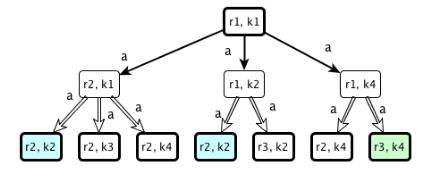
\includegraphics[scale = 0.6]{img/alb1.jpg}
  \end{figure}
\end{esempio}
\begin{esempio}
  Vediamo l'esempio di un gioco con due processi che dimostreremo non essere
  bisimili:\\

  Siano:
  \[q_1=a\cdot b\cdot Nil+a\cdot c\cdot Nil\]
  ovvero:
  \begin{center}
    \begin{tikzpicture}[shorten >=1pt,node distance=2cm,on grid,auto] 
      \node[state] (q_0) {$q_1$};  
      \node[state] (q_1) [below left =of q_0] {$q_2$};
      \node[state] (q_2) [below right =of q_0] {$q_3$};
      \node[state] (q_3) [below right =of q_1] {$Nil$};
      \path[->]
      (q_0) edge [above left] node {$a$} (q_1)
      (q_0) edge  node {$a$} (q_2)
      (q_1) edge [below left] node {$b$} (q_3)
      (q_2) edge  node {$c$} (q_3)
      ;
    \end{tikzpicture}
  \end{center}
 
  e:
  \[u_1=a\cdot (\tau\cdot b\cdot Nil+\tau\cdot c\cdot Nil)\]
  ovvero:
   \begin{center}
     \begin{tikzpicture}[shorten >=1pt,node distance=2cm,on grid,auto]
      
      \node[state] (q_0) {$u_2$};  
      \node[state] (q_1) [below left =of q_0] {$u_3$};
      \node[state] (q_2) [below right =of q_0] {$u_4$};
      \node[state] (q_3) [below right =of q_1] {$Nil$};
      \node[state] (q_4)[above =of q_0]  {$u_1$}; 
      \path[->]
      (q_0) edge [above left] node {$\tau$} (q_1)
      (q_0) edge  node {$\tau$} (q_2)
      (q_1) edge [below left] node {$b$} (q_3)
      (q_2) edge  node {$c$} (q_3)
      (q_4) edge  node {$a$} (q_0)
      ;
    \end{tikzpicture}
  \end{center}
  Vediamo quindi come si svolgono tutte le partite per $G(q_1,u_1)$.\\
  L'attaccante esegue $u_1\stackrel{a}{\rightarrow}u_2$.\\
  Il difensore ha due scelte:
  \begin{itemize}
    \item $q_1\stackrel{a}{\rightarrow}q_2$. Sono quindi in $(q_2,u_2)$. A
    questo punto $u_2\stackrel{\tau}{\rightarrow}u_4$ a cui il difensore non
    può che rispondere con l’azione nulla, $q_2\stackrel{\tau}{\rightarrow}q_2$,
    perdendo in quanto $q_2\not\approx^{Bis} u_4$ dato che dal primo, $q_2$
    posso fare solo $b$ e dal secondo, $u_4$ solo $c$ 
    
    
    \item $q_1\stackrel{a}{\rightarrow}q_3$. Sono quindi in $(q_3,u_2)$. A
    questo punto $u_2\stackrel{\tau}{\rightarrow}u_3$ a cui il difensore non
    può che rispondere con l’azione nulla, $q_3\stackrel{\tau}{\rightarrow}q_3$,
    perdendo in quanto $q_3\not\approx^{Bis} u_3$ dato che dal primo, $q_3$,
    posso fare solo $c$ e dal secondo, $u_3$, solo $b$
  \end{itemize}
  Quindi:
  \[q_1\not\approx^{Bis} u_1\]
  Vediamo anche in questo caso un albero parziale, dove si vedono anche le mosse
  in cui l'attaccante perdeva. Sono di egual colore le configurazioni identiche
  e si hanno col bordo bold le foglie (non colorate) corrispondi alle vincite
  del difensore, 
  che però non ha sempre una mossa per risponde attaccante, comportando la non
  bisimulazione:
  
  \begin{figure}[H]
    \centering
    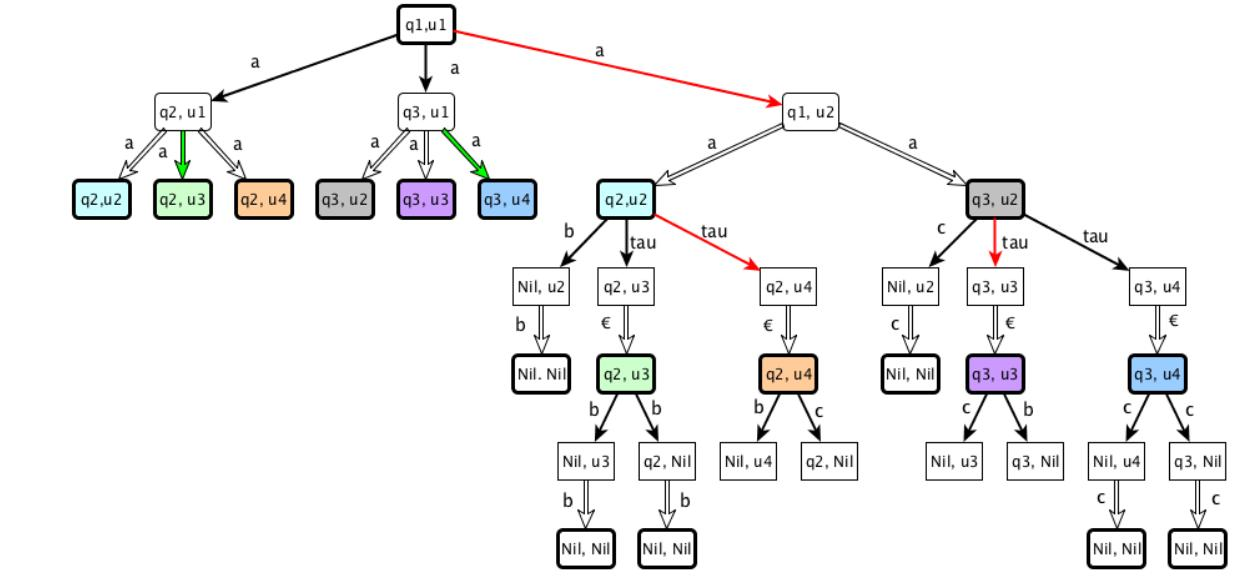
\includegraphics[scale = 0.31]{img/alb2.jpg}
  \end{figure}
  Si hanno infatti 4 foglie non colorate e non con il contorno bold che
  segnalano la vittoria dell'attaccante.\\
  Le foglie colorate rappresentano parti di alberi parziali.
\end{esempio}
\begin{itemize}
  \item se sono bisimili il difensore deve poter trovare una mossa vincente per
  ogni mossa dell'attaccante e quindi per ogni possibile mossa intermedia,
  avendo quindi una strategia vincente
  \item se non sono bisimili si ha almeno una mossa dell'attaccante, in ogni
  configurazione, per cui, comunque scelga poi il difensore, l'attaccante avrà
  ancora una mossa vincente, avendo quindi una strategia vincente
\end{itemize}
\textit{Se non si vuole dimostrare la bisimilitudine ma la si vuole cercare da
  zero bisogna studiare tutte le possibili partite o, meglio, un insieme di
  partite che mi possa dimostrare quale dei due giocatori ha la
  \textbf{strategia vincente}.}\\
Facciamo un piccolo ``recap'' della situazione.
\begin{definizione}
  Definiamo una \textbf{proprietà di equivalenza} tra processi CCS:
  \[\backsimeq \,\,\subseteq  Proc_{CCS}\times  Proc_{CCS}\]
  Si ha che, dati $p,q\in Proc_{CCS}$:
  \[\mbox{se }LTS(p)=LTS(q)\mbox{ allora } p\backsimeq q\]
  (ovvero se i due LTS sono isomorfi)\\
  Vale per altri modelli di concorrenza oltre che a il CCS.\\
  Si stanno considerando solo le azioni e non gli stati (si hanno altri approcci
  che considerano gli stati).
\end{definizione}
\begin{teorema}
  Si ha che, dati $p,q\in Proc_{CCS}$:
  \[p\backsimeq q\implies Tracce(p)=Tracce(q)\]
  Qui le stesse sequenze di azioni possono essere eseguite su entrambi i
  processi.  
\end{teorema}
\begin{teorema}
  Si ha che, dati $\forall p,q\in Proc_{CCS}$, qualora si abbia che $p\backsimeq
  q$, i due processi devono avere la stessa possibilità di generare deadlock
  nell'interazione con l'ambiente (ovvero l'insieme dei processi con cui $p$ e
  $q$ possono interagire). Quindi sostituendo $p$ con $q$, qualora il
  primo non avesse deadlock, posso dire che anche il secondo non avrà deadlock
  se questi sono equivalenti.
\end{teorema}
\begin{teorema}
  Si ha che $\backsimeq$ deve essere una \textbf{congruenza} rispetto agli
  operatori del CCS. Deve essere possibile sostituire un sottoprocesso con un
  suo equivalente senza modificare il comportamento complessivo del
  sistema. Sostituendo quindi un sottoprocesso con un suo equivalente il
  processo di partenza deve essere equivalente al nuovo processo ottenuto dopo
  la sostituzione, in qualsiasi contesto ci si trovi.
\end{teorema}
\begin{definizione}
  Definiamo l'\textbf{equivalenza rispetto alle tracce forte} $\sim^T$. Dati
  $\forall p,q\in Proc_{CCS}$:
  \[LTS(p)=LTS(q)\implies p\sim^T q\]
  Anche qui si estrae dagli stati, osservando solo le tracce, e si ha che:
  \[p\sim^T q\iff Tracce(p)=Tracce(q)\]
\end{definizione}
\begin{teorema}
  Si dimostra che l'equivalenza rispetto alle tracce forte è una
  \textbf{congruenza} rispetto agli operatori CCS.
\end{teorema}
\begin{teorema}
  La nozione di equivalenza rispetto alle tracce forte non garantisce di
  preservare il deadlock o l'assenza di deadlock nell'interazione con l'ambiente
  (come visto nell'esempio \ref{coffe}, dove l'equivalenza rispetto alle tracce
  forte non è sufficiente a garantire nulla rispetto al deadlock).
\end{teorema}
Partendo da quanto sopra si introduce quindi concetto di \textbf{bisimulazione
  forte} (equivalenza forte rispetto alla bisimulazione), introdotto da
Milner. Si ricorda che, $\forall p,q\in Proc_{CCS}$, 
astraendo dagli stati:
\begin{itemize}
  \item $LTS(p)=LTS(q)\implies p\sim^{Bis}q$
  
  \item $p\sim^{Bis}q\implies Tracce(p)=Tracce(q)$. In altri termini si ha che
  $p\sim^{Bis}q\implies p\sim^T q$ e quindi:
  \[\sim^{Bis}\subseteq \sim^T\]
  non posso avere processi bisimili che non abbiano le stesse tracce
  \item la bisimulazione forte preserva il deadlock o l'assenza di deadlock
  nell'interazione con l'ambiente
  \item la bisimulazione forte è una congruenza rispetto agli operatori del CCS
\end{itemize}
Si ha però che la bisimulazione forte è troppo restrittiva infatti, come anche
$\sim^T$, non astrae $\tau$, avendo, per esempio, che $a\cdot b\cdot
Nil\not\sim^{Bis} a\cdot \tau\cdot b\cdot Nil$. Non posso quindi confrontare
alcuna specifica con sincronizzazioni interne alle componenti di un processo,
rispetto alle azioni non osservabili.\\ 
Si è introdotta quindi la regola di \textbf{transizione debole},
$\stackrel{a}{\Rightarrow}$.\\ 
Si ha \textbf{l'equivalenza debole rispetto alle tracce}, $\approx^T$ è meno
restrittiva rispetto a quella forte infatti:
\[p\sim^T q\implies p\approx^T q\]
e quindi:
\[\sim^T \subseteq \approx^T\]
Quindi se due processi sono equivalenti fortemente rispetto alle tracce lo
saranno anche debolmente. L'equivalenza debole rispetto alle tracce ha quindi le
seguenti proprietà, astraendo dagli stati:
\begin{itemize}
  \item $LTS(p)=LTS(q)\implies p\approx^{T}q$
  \item l'equivalenza debole rispetto alle tracce è una congruenza rispetto
  agli operatori del CCS 
  \item l'equivalenza debole rispetto alle tracce non garantisce di
  preservare il deadlock o l'assenza di deadlock nell'interazione con l'ambiente
\end{itemize}
Passando alla \textbf{bisimulazione debole} (equivalenza debole rispetto alla
bisimulazione), $\approx^{Bis}$ si ha che è meno 
restrittiva rispetto a quella forte infatti:
\[p\sim^{Bis} q\implies p\approx^{Bis} q\]
e quindi:
\[\sim^{Bis} \subseteq \approx^{Bis}\]
Si ha quindi che la bisimulazione forte è più restrittiva ell’equivalenza
rispetto alle tracce forte ed egualmente la bisimulazione debole è più
restrittiva ell’equivalenza rispetto alle tracce debole:
\[p\sim^{Bis}q\implies p\sim^T q\mbox{ e }p\approx^{Bis}q\implies p\approx^Tq\]
quindi si ha che:
\[\sim^{Bis}\subseteq\sim^T \mbox{ e }\approx^{Bis}\subseteq\approx^T\]
Non si hanno rapporti ``misti'' tra forte e debole.\\

\begin{definizione}
  Dato $p\in Proc_{CCS}$ si ha che esso è un \textbf{processo deterministico}
  sse vale che:
  \[\forall x\in Act,\mbox{se } p\stackrel{x}{\rightarrow}p'\mbox{ e
    }p\stackrel{x}{\rightarrow}p''\mbox{ allora }p'=p''\]
  Quindi se posso passare a $p'$ o $p''$ con la stessa azione allora
  necessariamente questi due processi coincidono.
\end{definizione}
\begin{esempio}
  vediamo un esempio di $p$ \textbf{non deterministico}:
  \[p=x\cdot p'+x\cdot p''\]
\end{esempio}
\begin{teorema}
  Siano $p,q\in Proc_{CCS}$ \textbf{deterministici} e sia $p\sim^Tq$ (quindi
  anche $p\approx^Tq$) allora si ha che:
  \[p\sim^{Bis}q\]
  e quindi anche:
  \[p\approx^{Bis}q\]
\end{teorema}
Avere processi deterministici con le stesse tracce non assicura che i due
processi abbiano lo stesso LTS. Come esempio basta vedere un processo $p=a\cdot
b\cdot a\cdot b\cdot p$ e uno $q=a\cdot b\cdot q$, dove il primo ha due nodi in
più anche se sono deterministici con quindi equivalenza rispetto alle tracce e
forte bisimilitudine, essendo quindi equivalenti, per entrambe le equivalenza,
debolmente.\\ 
Se ho invece due processi non entrambi deterministici potrei avere equivalenza
rispetto alle tracce (debole e forte) ma non bisimilitudine. Come esempio si
prendano $p=a\cdot \tau\cdot b\cdot Nil$ e $q=a\cdot(\tau\cdot b\cdot Nil+\tau
\cdot Nil)$, con quest'ultimo che non è un processo deterministico.\\
Basta quindi che un processo sia non deterministico per impedire il ``collasso''
dell'equivalenza rispetto alle tracce su quella rispetto alla bisimulazione.\\
Approfondiamo ora le proprietà della bisimulazione debole, tra cui:
\begin{itemize}
  \item la bisimulazione debole, per come è definita (unione di tutte le
  relazioni di bisimulazione), è la più grande relazione di bisimulazione debole
  ed è di equivalenza, essendo:
  \begin{itemize}
    \item riflessiva
    \item simmetrica
    \item transitiva
  \end{itemize}
  \item la bisimulazione debole, come quella forte, preserva la possibilità di
  generare o meno deadlock nell'interazione con l'ambiente, quindi sostituendo
  un processo che non genera deadlock con un suo bisimile ho che anche il nuovo
  sistema non andrà in deadlock (se invece generava un deadlock ora andrà
  in deadlock). Questa cosa, si ricorda, non è vera per le l'equivalenza sulle
  tracce
  
  \item la bisimulazione debole, a differenza di quella forte, astrae da azioni
  non osservabili, le $\tau$, e da cicli inosservabili, i $\tau$ loop. Se ho un
  ciclo infinito di $\tau$ si parla di \textbf{divergenza}.
  \begin{esempio}
    Presi un processo $Nil$ e uno $p=\tau\cdot p$ (quindi un processo infinito
    di sole $\tau$, una divergenza) ho che:
    \[Nil\approx^{Bis}p\]
    avendo:
    \begin{center}
      \begin{tikzpicture}[shorten >=1pt,node distance=2cm,on grid,auto] 
        \node[state] (q_0) {$p$};  
        \node[state] (q_3) [left =of q_0] {$Nil$};
        \path[->]
        (q_0) edge [loop right] node {$\tau$} (q_0)
        ;
      \end{tikzpicture}
    \end{center}
  \end{esempio}
  \begin{esempio}
    Siano $q=a\cdot b\cdot Nil$ e $s\cdot a\cdot v$ con $v=\tau\cdot v+b\cdot
    Nil$. Ho che:
    \[q\approx^{Bis} s\]
    ma:
    \[q\not\sim^{Bis} s\]

    avendo:
    \begin{center}
      \begin{tikzpicture}[shorten >=1pt,node distance=2cm,on grid,auto] 
        \node[state] (q_0) {$q$};  
        \node[state] (q_1) [right =of q_0] {$b\cdot Nil$};
        \node[state] (q_2) [right =of q_1] {$Nil$};
        \path[->]
        (q_0) edge  node {$a$} (q_1)
        (q_1) edge node {$b$} (q_2)
        ;
      \end{tikzpicture}
    \end{center}
    e
    \begin{center}
      \begin{tikzpicture}[shorten >=1pt,node distance=2cm,on grid,auto] 
        \node[state] (q_0) {$s$};  
        \node[state] (q_1) [right =of q_0] {$v$};
        \node[state] (q_2) [right =of q_1] {$Nil$};
        \path[->]
        (q_0) edge  node {$a$} (q_1)
        (q_1) edge node {$b$} (q_2)
        (q_1) edge [loop above] node {$\tau$} (q_1)
        ;
      \end{tikzpicture}
    \end{center}
  \end{esempio}
  \begin{esempio}
    Presi $q=a\cdot b\cdot Nil$, $r=a\cdot(\tau\cdot p+b\cdot Nil)$ e $s\cdot
    a\cdot v$ con $v=\tau\cdot v+b\cdot 
    Nil$. Ho che:
    \[q\not\approx^{Bis}r\]
    \[s\not\approx^{Bis}r\]
    \newpage
    avendo, oltre ai due LTS dell'esercizio precedente:
    \begin{center}
      \begin{tikzpicture}[shorten >=1pt,node distance=3cm,on grid,auto] 
        \node[state] (q_0) {$r$};  
        \node[state] (q_1) [right =of q_0] {$\tau\cdot p+b\cdot Nil$};
        \node[state] (q_2) [right =of q_1] {$Nil$};
        \node[state] (q_3) [above =of q_1] {$p$};
        \path[->]
        (q_0) edge  node {$a$} (q_1)
        (q_1) edge node {$b$} (q_2)
        (q_1) edge node {$\tau$} (q_3)
        (q_3) edge [loop above] node {$\tau$} (q_3)
        ;
      \end{tikzpicture}
    \end{center}
  \end{esempio}
\end{itemize}
Ci si chiede quindi se la bisimulazione debole sia o meno una congruenza
rispetto agli operatori del CCS.\\
Si ricorda che:
\begin{definizione}
  Data una relazione di equivalenza $R\subseteq Proc_{CCS}\times Proc_{CCS}$
  essa è una congruenza se $\forall C[\cdot]$, contesto CCS con una certa
  variabile non specificata ``$\cdot$'', presi $p,q\in Proc_{CCS}$, ho che:
  \[pRq\implies C[p]\,\,R\,\,C[q]\]
  Quindi comunque prendo una specifica CCS posso sostituire a piacere i due
  processi. 
\end{definizione}
\begin{teorema}
  Si ha che $\forall\,p,q\in Proc_{CCS}$ se $p\approx^{Bis}q$, allora:
  \begin{itemize}
    \item $a\cdot p\approx^{Bis} a\cdot q,\forall\, a\in
    Act=A\cup\overline{A}\cup\{\tau\}$ 
    \item $p|r\approx^{Bis}q|r\,\,\,\land \,\,\,
    r|p\approx^{Bis}r|q,\forall\,r\in Proc_{CCS}$  
    \item $p[f]\approx^{Bis}q[f],\forall\,f\mbox{ funzione di rietichettatura}$,
    ricordando che la funzione preserva nomi, co-nomi (quindi l'immagine di un
    co-nome è uguale al co-nome dell'immagine) e $\tau$
    \item $p_{\backslash L}\approx^{Bis}q_{\backslash L},\forall\,L\subseteq A$,
    ricordando che la restrizione rispetto a $L$ comporta che il processo può
    eseguire le azioni in $L$ solo se sono sincronizzazioni interne
  \end{itemize}
\end{teorema}
Si nota che nel teorema precedente abbiamo, in ordine:
\begin{itemize}
  \item prefisso
  \item composizione parallela
  \item rietichettatura
  \item restrizione
\end{itemize}
Non si parla quindi dell'operatore di scelta ``+'' che infatti necessita di
ulteriori approfondimenti. Vediamo un esempio:
\begin{esempio}
  Possiamo, per esempio, dire che:
  \[\tau\cdot a\cdot Nil\approx^{Bis}a\cdot Nil\]
  ma:
  \[\tau\cdot a\cdot Nil+b\cdot Nil\not\approx^{Bis}a\cdot Nil+b\cdot Nil\]
  graficamente si ha, per il primo:
  \begin{center}
    \begin{tikzpicture}[shorten >=1pt,node distance=3cm,on grid,auto] 
      \node[state] (q_0) {$p$};  
      \node[state] (q_1) [right =of q_0] {$a\cdot Nil$};
      \node[state] (q_2) [right =of q_1] {$Nil$};
      \path[->]
      (q_0) edge  node {$\tau$} (q_1)
      (q_1) edge node {$a$} (q_2)
      ;
    \end{tikzpicture}
  \end{center}
  e:
  \begin{center}
    \begin{tikzpicture}[shorten >=1pt,node distance=3cm,on grid,auto] 
      \node[state] (q_0) {$q$};  
      \node[state] (q_2) [right =of q_0] {$Nil$};
      \path[->]
      (q_0) edge  node {$a$} (q_2)
      ;
    \end{tikzpicture}
  \end{center}
  ma componendo $r=b\cdot Nil$ ottengo:
  \begin{center}
    \begin{tikzpicture}[shorten >=1pt,node distance=3cm,on grid,auto] 
      \node[state] (q_0) {$p+r$};  
      \node[state] (q_1) [right =of q_0] {$a\cdot Nil$};
      \node[state] (q_2) [right =of q_1] {$Nil$};
      \path[->]
      (q_0) edge  node {$\tau$} (q_1)
      (q_1) edge node {$a$} (q_2)
      (q_0) edge [bend left=45]  node {$b$} (q_2)
      ;
    \end{tikzpicture}
  \end{center}
  e:
  \begin{center}
    \begin{tikzpicture}[shorten >=1pt,node distance=3cm,on grid,auto] 
      \node[state] (q_0) {$q+r$};  
      \node[state] (q_2) [right =of q_0] {$Nil$};
      \path[->]
      (q_0) edge [bend left]  node {$a$} (q_2)
      (q_0) edge [bend right]  node [below] {$b$} (q_2)
      ;
    \end{tikzpicture}
  \end{center}
  vedendo che non sono bisimili perché $a\cdot Nil$ non può avere corrispondenti
  nel secondo LTS.
\end{esempio}
Si ha quindi che la \textbf{bisimulazione debole non è una congruenza per il
  CCS}, a differenza di quella forte (secondo la quale, nell'esempio precedente,
avremmo avuto direttamente $p\not\sim^{Bis}q$), in quanto non è una congruenza
rispetto alla scelta.\\
Si ha inoltre che la bisimulazione debole non è una congruenza rispetto alla
\textbf{ricorsione} (anche se non dimostriamo la cosa).\\
Possiamo quindi dire che la \textbf{bisimulazione debole è una congruenza
  rispetto agli operatori del CCS diversi da scelta e ricorsione.}\\
Vogliamo quindi identificare una relazione di congruenza, che è sempre una
relazione binaria tra processi CCS, che sia la più grande relazione contenuta
nella bisimulazione che sia però una congruenza rispetto a tutti gli
operatori:
\[\approx^C\subseteq\approx^{Bis}\subseteq Proc_{CCS}\times Proc_{CCS}\]
Per il CCS puro senza ricorsione Milner ha introdotto un insieme
finito di assiomi che possono essere visti come regole di riscrittura che
preservano la \textbf{congruenza all'osservazione}, che è la più grande
congruenza contenuta nella bisimulazione. Questo insieme di assiomi è quindi un
insieme finito per il quale, presi due processi $p,q\in Proc_{CCS}$, se riesco,
tramite questi assiomi, a trasformare l'uno nell'altro allora si ha che questi
processi non sono solo bisimili ma anche congruenti (potendo quindi sostituire
l'uno con l'altro in qualsiasi contesto che non includa la ricorsione). Questo
insieme di assiomi, detto $Ax$, è:
\begin{itemize}
  \item \textbf{corretto}, ovvero che se usando l'insieme di assiomi deduco che
  $p=q$ allora $p$ è congruente a $q$ rispetto a questa nuova nozione si
  congruenza:
  \[Ax\vdash p=q\implies p\approx^C q\]
  \item \textbf{completo}, ovvero presi due processi che sono congruenti secondo
  questa nuova nozione di congruenza allora sicuramente questo insieme di
  assiomi è completo in quanto mi permette, tale insieme, di trascrivere $p$ in
  $q$, ovvero:
  \[p\approx^C q\implies AX\vdash p=q\]
\end{itemize}
Vediamo quindi questi assiomi:
\begin{itemize}
  \item $p+(q+r)\approx^C (p+q)+r$ e $p|(q|r)\approx^C (p|q)|r$, ovvero
  l'assioma riguardo l'associatività di scelta e composizione parallela
  \item $p+q\approx^C q+p$ e $p|q\approx^Cq|p$, ovvero
  l'assioma riguardo la commutatività di scelta e composizione parallela
  \item $p+p\approx^C p$ ma $p|p\not\approx^C p$, ovvero si ha l'assioma per
  l'assorbimento riguardo la scelta ma non si ha riguardo la composizione
  parallela (si pensi per esempio a $p=\cdot Nil$ avrei $a$ due volte mentre $p$
  può fare $a$ una volta sola)  
  \item $p+Nil\approx^C p$ e $p|Nil \approx^Cp$, ovvero ovvero si ha l'assioma
  per l'assorbimento del $Nil$ riguardo la scelta e la composizione parallela
  \item $p+\tau\cdot p\approx^C\tau\cdot p$, che è l'assioma che risolve il
  problema di avere una scelta con un una $\tau$ iniziale nella sequenza, che
  non può essere eliminata
  \item $\mu\cdot \tau\cdot p\approx \mu\cdot p,\,\,\,\forall\,\mu\in Act$, che
  tratta le $\tau$ interne alla sequenza, che può essere eliminata
  \item $\mu\cdot(p+\tau\cdot 1)\approx^C\mu\cdot(p+\tau\cdot q)+\mu\cdot q$,
  ovvero per questo assioma si ha che il primo che è una ``semplificazione''
  del secondo (intuizione da esempio)
\end{itemize}
\begin{esempio}
  Vediamo l'ultimo assioma con un esempio.\\
  Siano:
  \[r_1=a\cdot(b\cdot Nil+\tau\cdot c\cdot Nil)\]
  \[k_1=a\cdot(b\cdot Nil+\tau\cdot c\cdot Nil)+a\cdot c\cdot Nil\]
  ovvero:
  \begin{center}
    \begin{tikzpicture}[shorten >=1pt,node distance=2cm,on grid,auto] 
      \node[state] (q_0) {$r_1$};  
      \node[state] (q_1) [right =of q_0] {$r_2$};
      \node[state] (q_2) [right =of q_1] {$Nil$};
      \node[state] (q_3) [above =of q_1] {$r_3$};
      \path[->]
      (q_0) edge  node {$a$} (q_1)
      (q_1) edge node {$b$} (q_2)
      (q_1) edge node {$\tau$} (q_3)
      (q_3) edge node {$c$} (q_2)
      ;
    \end{tikzpicture}
  \end{center}
  \newpage
  e:
  \begin{center}
    \begin{tikzpicture}[shorten >=1pt,node distance=2.5cm,on grid,auto] 
      \node[state] (q_0) {$k_1$};  
      \node[state] (q_1) [above right =of q_0] {$k_4$};
      \node[state] (q_2) [below right =of q_0] {$k_2$};
      \node[state] (q_3) [right=of q_2] {$k_3$};
      \node[state] (q_4) [above right=of q_2] {$Nil$};
      \path[->]
      (q_0) edge  node {$a$} (q_1)
      (q_0) edge  node {$a$} (q_2)
      (q_2) edge node {$b$} (q_3)
      (q_2) edge node {$\tau$} (q_4)
      (q_1) edge node {$c$} (q_4)
      (q_3) edge node {$c$} (q_4)
      ;
    \end{tikzpicture}
  \end{center}
  e si ha vede che:
  \[r_1\approx^C k_1\]
  con il primo che è una ``semplificazione'' del secondo.
\end{esempio}
Si hanno anche altri assiomi legati al fatto che $p$ e $q$ siano delle somme,
ovvero:
\[p=\sum_i a_i\cdot p_i,\,\,\,a\in Act\]
\[q=\sum_j b_j\cdot q_j,\,\,\,b\in Act\]
avendo quindi i seguenti assiomi:
\begin{itemize}
  \item $p|q\approx^C\sum_i a_i\cdot (p_i|q)+\sum_j b_j\cdot
  (p|q_j)+\sum_{a_i=\overline{b_j}}\tau\cdot(p_i|q_j)$ che è l'assioma detto
  \textbf{teorema di espansione di Milner} (nell'ultima parte ho che se $a_i$ e
  $b_j$ sono l'uno il complemento dell'altro allora posso sincronizzare su di
  essi i processi, che diventano una $\tau$ e proseguendo con $p_i|q_j$). È la
  generalizzazione dell'operatore parallelo con la regola d'inferenza vista ad
  inizio capitolo.
  \item $p[f]\approx^C \sum_if(a_i)\cdot(p_i[f]),\,\,\,\forall\,f\mbox{ funzione
    di etichettatura}$, ovvero etichettare tutto il processo $p$ corrisponde al
  fatto di ottenere congruo il processo che ottengo etichettando ogni i-sima
  azione delle componenti che sono in alternativa con il processo relativo
  rietichettato con $f$
  \item $p_{\backslash L}\approx^C \sum_{a_i,\overline{a_i}\not\in
    L}a_i\cdot(p_{i\backslash L}),\,\,\,\forall\,L\subseteq A$ quindi considero
  solo le azioni per le quali non si ha al restrizione
\end{itemize}
Per cui la bisimulazione risulta tale per cui se usiamo $\approx^C$ si può
modellare un sistema a passi successivi sapendo che posso sostituire un
sottoprocesso con un altro ottenendo ancora un sistema bisimile al precedente.
\begin{esempio}
  Vediamo un esempio sull'assioma detto \textbf{teorema di espansione}.\\
  Si ha, sviluppando a partire dal primo:
  \[a\cdot c\cdot Nil|b\cdot Nil\approx^C\]
  \[a\cdot(c\cdot NIl|b\cdot Nil)+b\cdot(a\cdot c \cdot Nil|Nil)\approx^C\]

  \[a\cdot(c\cdot(Nil|b\cdot Nil)+b\cdot(c\cdot Nil|Nil))+b\cdot(a\cdot(c\cdot
    Nil|Nil))\approx^C\]
  \[a\cdot (c\cdot b\cdot(NIl|Nil)+b\cdot c\cdot(Nil|NIl))+b\cdot(a\cdot
    c\cdot(Nil|Nil))\approx^C\]
  \[a\cdot(c\cdot b\cdot Nil+b\cdot c\cdot Nil)+b\cdot a\cdot c\cdot Nil\]
  e quindi:
  \[a\cdot c\cdot Nil|b\cdot Nil\approx^Ca\cdot(c\cdot b\cdot Nil+b\cdot c\cdot
    Nil)+b\cdot a\cdot c\cdot Nil\]
  infatti si ha:
   \begin{center}
    \begin{tikzpicture}[shorten >=1pt,node distance=4cm,on grid,auto] 
      \node[elliptic state] (q_0) {$a\cdot c\cdot Nil |b\cdot Nil$};  
      \node[elliptic state] (q_1) [below left =of q_0] {$c\cdot Nil|b\cdot Nil$};
      \node[elliptic state] (q_2) [below right =of q_0] {$a\cdot c\cdot Nil|Nil$};
      \node[elliptic state] (q_3) [below left=of q_2] {$c\cdot Nil|Nil$};
      \node[elliptic state] (q_4) [below=of q_1] {$Nil|b\cdot Nil$};
      \node[elliptic state] (q_5) [below right=of q_4] {$Nil$};
      \path[->]
      (q_0) edge [above left] node {$a$} (q_1)
      (q_0) edge  node {$b$} (q_2)
      (q_1) edge [below left]node {$b$} (q_3)
      (q_1) edge node {$c$} (q_4)
      (q_2) edge node {$a$} (q_3)
      (q_3) edge node {$c$} (q_5)
      (q_4) edge node {$b$} (q_5)
      ;
    \end{tikzpicture}
  \end{center}
\end{esempio}
\begin{esempio}
  Vediamo l'esempio della \textbf{mutua esclusione} con la primitiva di un
  \textbf{semaforo}. \\
  Si ha la specifica:
  \[spec=b_1\cdot e_1\cdot spec+b_2\cdot e_2\cdot spec\]
  \begin{center}
    \begin{tikzpicture}[shorten >=1pt,node distance=3cm,on grid,auto] 
      \node[elliptic state] (q_0) {$spec$};  
      \node[elliptic state] (q_1) [below left =of q_0] {$e_1\cdot spec$};
      \node[elliptic state] (q_2) [below right =of q_0] {$e_2\cdot spec$};
      \path[->]
      (q_0) edge [bend right = 25] node [above left]{$b_1$} (q_1)
      (q_0) edge [bend left= 25] node {$b_2$} (q_2)
      (q_1) edge [bend right = 25] node [below right] {$e_1$} (q_0)
      (q_2) edge [bend left= 25] node {$e_2$} (q_0)
      ;
    \end{tikzpicture}
  \end{center}
  e l'implementazione:
  \[sys=(A_1|S|A_2)_{\backslash\{p,v\}}\]

  con:
  \[S=p\cdot v\cdot S\]
  \begin{center}
    \begin{tikzpicture}[shorten >=1pt,node distance=2cm,on grid,auto] 
      \node[state] (q_0) {$S$};  
      \node[state] (q_1) [below =of q_0] {$v\cdot S$};
      \path[->]
      (q_0) edge [bend right = 25] node [above left]{$p$} (q_1)

      (q_1) edge [bend right = 25] node [below right] {$v$} (q_0)
      ;
    \end{tikzpicture}
  \end{center}
  e con:
  \[A_1=\overline{p}\cdot b_2\cdot e_1\cdot \overline{v}\cdot A_1\]
  \[A_2=\overline{p}\cdot b_2\cdot e_2\cdot \overline{v}\cdot A_2\]
  \begin{center}
    \begin{tikzpicture}[shorten >=1pt,node distance=2cm,on grid,auto] 
      \node[elliptic state] (q_0) {$A_1$};  
      \node[elliptic state] (q_1) [below =of q_0] {$b_i\cdot
        e_i\cdot\overline{v}\cdot A_i$}; 
      \node[elliptic state] (q_2) [below =of q_1] {$e_i\cdot \overline{v}\cdot
        A_i$}; 
      \node[elliptic state](q_3) [below =of q_2] {$\overline{v}\cdot A_i$};
      \path[->]
      (q_0) edge node {$\overline{p}$} (q_1)
      (q_1) edge node {$b_i$} (q_2)
      (q_2) edge node {$e_i$} (q_3)
      (q_3) edge [bend right = 65]node [right]{$\overline{v}$} (q_0)
      ;
    \end{tikzpicture}
  \end{center}
  Si ha quindi:
  \begin{center}
    \begin{tikzpicture}[shorten >=1pt,node distance=5cm,on grid,auto] 
      \node (q_0) {$(A_1|S|A_2)_{\backslash\{p,v\}}$};  
      \node (q_1) [below left =of q_0] {$(b_1\cdot e_1\cdot \overline{v}\cdot
        A_1|v\cdot S|A_2)_{\backslash\{p,v\}}$};
      \node (q_2) [below right =of q_0] {$(A_1|v\cdot S|b_2\cdot e_2\cdot
        \overline{v}\cdot A_2)_{\backslash\{p,v\}}$};
      \node (q_3) [below =of q_1] {$(e_1\cdot \overline{v}\cdot
        A_1|v\cdot S|A_2)_{\backslash\{p,v\}}$};
      \node (q_4) [below =of q_3] {$\overline{v}\cdot
        A_1|v\cdot S|A_2)_{\backslash\{p,v\}}$};
      \node (q_5) [below =of q_2] {$(A_1|v\cdot S| e_2\cdot
        \overline{v}\cdot A_2)_{\backslash\{p,v\}}$};
      \node (q_6) [below =of q_5] {$(\overline{v}\cdot A_2)_{\backslash\{p,v\}}$};
      \path[->]
      (q_0) edge node [above left] {$\tau$} (q_1)
      (q_0) edge node {$\tau$} (q_2)
      (q_1) edge node {$b_1$} (q_3)
      (q_3) edge node {$e_1$} (q_4)
      (q_2) edge node {$b_2$} (q_5)
      (q_5) edge node {$e_2$} (q_6)
      (q_6) edge [bend left = 20] node [above right]{$\tau$} (q_0)
      (q_4) edge [bend right = 20] node {$\tau$} (q_0)
      ;
    \end{tikzpicture}
  \end{center}
  Vedo se $spec\approx^{Bis}sys$ ma ho che l'attaccante ha una strategia
  vincente, fa una $\tau$ sul primo processo in $sys$. Nella seconda mossa poi
  l'attaccante opera su $spec$ facendo $b_2$ e il difensore perde:
  \[spec\not\approx^{Bis}sys\]
\end{esempio}
\textbf{altri esempi su slide.}\\
Dati due processi $p_1$ e $p_2$ abbiamo che la composizione parallela è detta a
\textbf{semantica interleaving}, in quanto si vede dalle regole di inferenza che
posso eseguire o uno o l'altro o sincronizzare, grazie all'assunzione
dell'atomicità delle azioni
La cosa è visibile per esempio con:
\[p=a\cdot Nil|b\cdot Nil\]
\[q=a\cdot b\cdot Nil+b\cdot a\cdot Nil\]
Avendo:
\[p\sim^{Bis}q\]
Togliendo l'atomicità, mettendo $a$ come $a_1,a_2$ si ha:
\[p'=p_{\left[a \leftarrow a_{1} \cdot a_{2}\right]}=a_{1} \cdot a_{2}
  \cdot N i l \mid b . N i l \]
\[      q'=q_{\left[a \leftarrow a_{1}, a_{2}\right]}=a_{1} \cdot a_{2}
  \cdot b \cdot N i l+b \cdot a_{1} \cdot a_{2} \cdot N i l\]
Avendo:
\begin{center}
  \begin{tikzpicture}[shorten >=1pt,node distance=3cm,on grid,auto] 
    \node[elliptic state] (q_0) {$p'$};  
    \node[elliptic state] (q_1) [below left =of q_0] {$a_2\cdot Nil|b\cdot
      Nil$};
    
    \node[elliptic state] (q_2) [below right =of q_0] {$a_1\cdot a_2\cdot
      Nil|Nil$};
    
    \node[elliptic state] (q_3) [below left=of q_2] {$a_2\cdot Nil|Nil$};
    \node[elliptic state] (q_4) [below=of q_1] {$Nil|b\cdot Nil$};
    \node[elliptic state] (q_5) [below right=of q_4] {$Nil| Nil$};
    \path[->]
    (q_0) edge [above left] node {$a_1$} (q_1)
    (q_0) edge  node {$b$} (q_2)
    (q_1) edge [below left]node {$b$} (q_3)
    (q_1) edge node {$a_2$} (q_4)
    (q_2) edge node {$a_1$} (q_3)
    (q_3) edge node {$a_2$} (q_5)
    (q_4) edge node {$b$} (q_5)
    ;
  \end{tikzpicture}
\end{center}
\newpage
e:
\begin{center}
  \begin{tikzpicture}[shorten >=1pt,node distance=3cm,on grid,auto] 
    \node[elliptic state] (q_0) {$p'$};  
    \node[elliptic state] (q_1) [below left =of q_0] {$a_2\cdot b\cdot
      Nil$};
    
    \node[elliptic state] (q_2) [below right =of q_0] {$a_1\cdot a_2\cdot
      Nil$};
    
    \node[elliptic state] (q_3) [below =of q_2] {$a_2\cdot Nil$};
    \node[elliptic state] (q_4) [below=of q_1] {$b\cdot Nil$};
    \node[elliptic state] (q_5) [below right=of q_4] {$Nil$};
    \path[->]
    (q_0) edge [above left] node {$a_1$} (q_1)
    (q_0) edge  node {$b$} (q_2)
    (q_1) edge node {$a_2$} (q_4)
    (q_2) edge node {$a_1$} (q_3)
    (q_3) edge node [above left] {$a_2$} (q_5)
    (q_4) edge node {$b$} (q_5)
    ;
  \end{tikzpicture}
\end{center}
e si ha che $p'\neq\sim^Tq'$. Se le azioni non sono più atomiche quindi
``rompo'' la composizione parallela, avrei bisogno infatti di una semantica
basata sulla \textbf{true concurrency}.\\
Nella letteratura è stata definita la bisimulazione definita differenziando
azioni concorrenti e in sequenza (per esempio tramite le reti di Petri, che si
basano sulla \textit{true concurrency}).\\
\textbf{Sulle slide esempio di un protocollo di comunicazione fatto con CCS e
  poi con reti di Petri e ulteriori esempi di partite per la bisimulazione}.